\documentclass{pl-slide}

\usepackage[british]{babel}
\usepackage[british]{datetime2}
\usepackage{ulem}

\usepackage{svg}

\usepackage{qrcode}
\usepackage{twemojis}

\usepackage{tikz,calc}
\usetikzlibrary{shapes}

\usetikzlibrary{shapes.geometric, shapes.multipart, arrows, chains, fit, quotes}

\settheme{ipfs-camp-2022}

%Information to be included in the title page:
%\title{Content Routing Privacy: Double Hashing}
%\subtitle{Double Privacy Benefits of Double Hashing}
%\title{Double Privacy Benefits of Double Hashing}
\title{Privacy \& libp2p}
\subtitle{Double Hashing in the DHT}
\author{Gui Michel}
\handle{@guissou}
\avatar{resources/avatar.png}
\group{ProbeLab}
\institute{Protocol Labs}
\event{IPFS Camp}
\date{\DTMdate{2022-10-30}}



\tikzstyle{dhtnode} = [rectangle, rounded corners, minimum width=3cm, minimum height=1cm, text centered, draw=text-color]

\tikzstyle{trienode} = [draw=text-color, rounded corners]

\tikzset{
state/.style={
       rectangle split,
       rectangle split parts=2,
       rounded corners,
       line width=1pt,
       draw=text-color,
       minimum height=10em,
       minimum width=15em,
       text width=14em,
       inner sep=2pt,
       text centered,
       }
}

\tikzset{
  basic box/.style = {
    shape = rectangle,
    align = center,
    draw  = #1,
    fill  = #1!25,
    rounded corners},
  header node/.style = {
    %Minimum Width = header nodes,
    font          = \strut\Large\ttfamily,
    text depth    = +0pt,
    fill          = white,
    draw},
  header/.style = {%
    inner ysep = +1.5em,
    append after command = {
      \pgfextra{\let\TikZlastnode\tikzlastnode}
      node [header node] (header-\TikZlastnode) at (\TikZlastnode.north) {#1}
      node at (0,0) (h-\TikZlastnode) {}
    }
  },
  hv/.style = {to path = {-|(\tikztotarget)\tikztonodes}},
  vh/.style = {to path = {|-(\tikztotarget)\tikztonodes}},
  fat blue line/.style = {ultra thick, blue}
}



\begin{document}

\frame{\titlepage}
\logo{
	\includegraphics[scale=0.1]{pl-resources/ipfs-camp-logo.png}
	\hspace{2em}
}

\begin{frame}
\frametitle{Agenda}
\begin{itemize}
	\itemc Goals
	\itemc DHT Content Routing in IPFS
	\itemc Double Hashing DHT Design
	\begin{itemize}
		\item[\greencube] Double Hash
		\item[\greencube] Prefix Lookup
		\item[\greencube] Provider Records Encryption
		\item[\greencube] Provider Records Authentication
	\end{itemize}
	\itemc Demo
	\itemc Transition
\end{itemize}
\end{frame}

\begin{frame}
\frametitle{Goals \& non-goals}

{\Large What this solution improves}
\begin{itemize}
	\itemc Reader Privacy when looking up content in the DHT
	\itemc From adversary able to observe network (e.g DHT server nodes)
\end{itemize}
\bigskip

{\Large What this solution does NOT target}
\begin{itemize}
	\itemc Writer Privacy in the DHT
	\itemc Data Transfer Privacy (e.g Bitswap)
\end{itemize}
\end{frame}

\begin{frame}
\frametitle{Privacy \& Content Routing - DHT Challenges}
\begin{itemize}
	\itemc \textbf{Content Routing} needs the content to be discoverable
	\begin{itemize}
		\item[\greencube] DHT server nodes need to know what you are looking for to help you find it
	\end{itemize}
		\bigskip
	\itemc \textbf{Privacy} needs the content to be private
	\begin{itemize}
		\item[\greencube] You don't want DHT server nodes to know which content you are looking for
	\end{itemize}

\end{itemize}
\end{frame}


\begin{frame}
\frametitle{Definitions}
{\Large
	MultiHash $\leftarrow$ Hash(\includegraphics[scale=0.03]{resources/image.png}):\hspace{1em}\texttt{mHash = 01010111}\\
	CID $\leftarrow$ \texttt{prefix0 + mHash = bafybeiaqr6csdcnxrkpx23...}\\
	Content second hash $\leftarrow$ Hash(\texttt{prefix1 + mHash}) = \texttt{10110001}\\
	\smallskip
	{\large\qquad\yellowcube\thinspace Note: \textit{For simplicity we represent the second hash as} \texttt{Hash(CID)}}\\
	\medskip
	Provider Record: Pointer \texttt{CID} $\rightarrow$ \texttt{PeerID} stored in the DHT
}


\end{frame}


\begin{frame}
\frametitle{Pinning content to the DHT}
\begin{minipage}[b]{\linewidth}
\begin{center}
	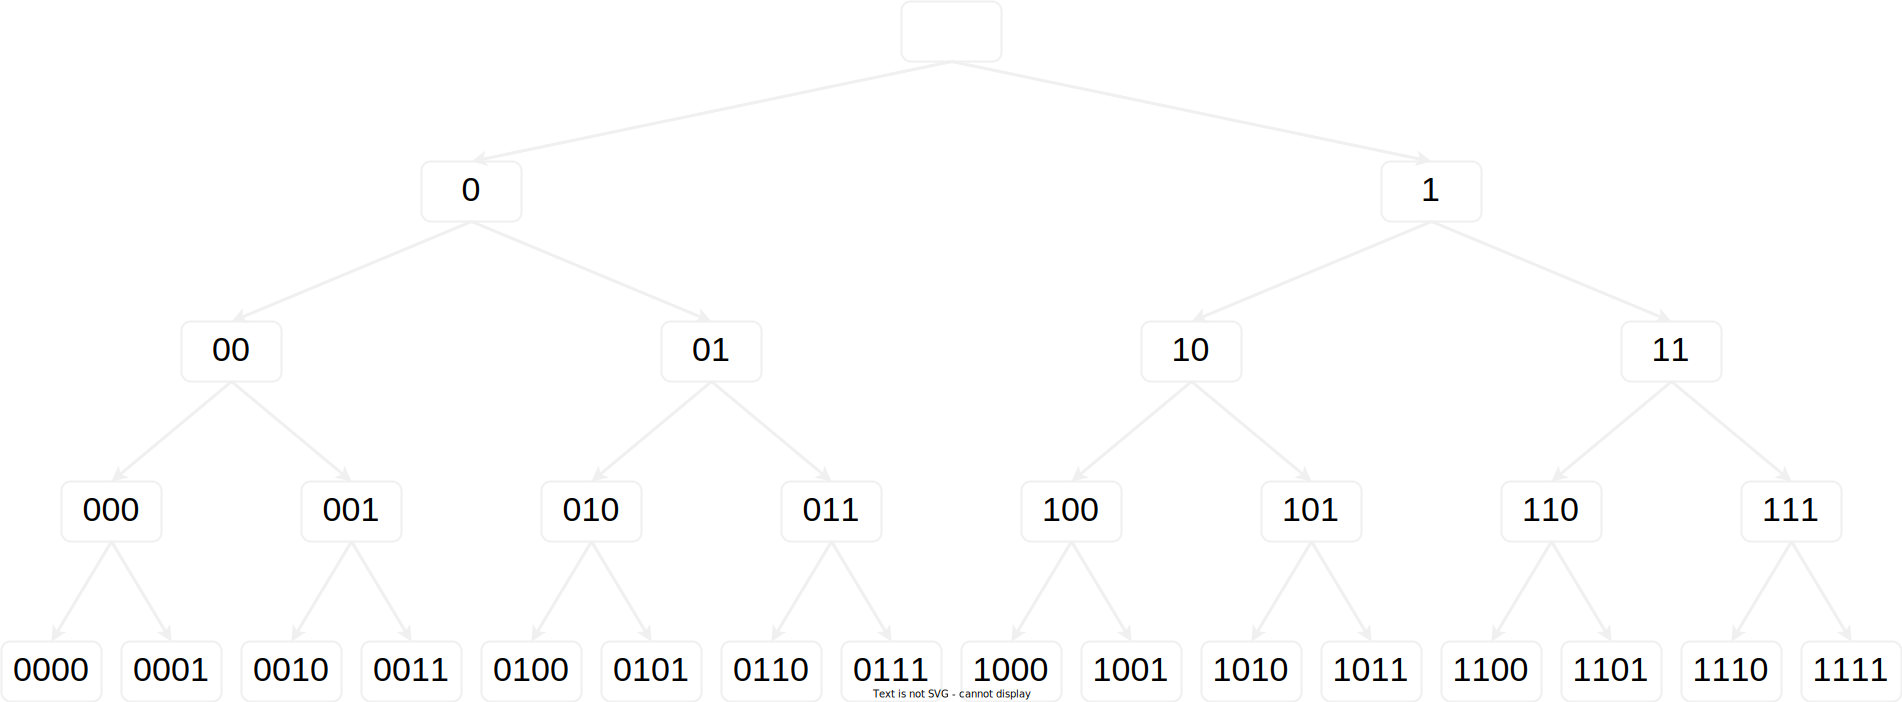
\includegraphics[width=.8\linewidth,keepaspectratio]{resources/dht/dht-vanilla.png}
\end{center}
\end{minipage}
\end{frame}

\begin{frame}
\frametitle{Pinning content to the DHT}
\begin{minipage}[b]{\linewidth}
\begin{center}
	\includegraphics[width=.8\linewidth,keepaspectratio]{resources/dht/dht-provider-lookup.png}
\end{center}
\end{minipage}
\end{frame}

\begin{frame}
\frametitle{Pinning content to the DHT}
\begin{minipage}[b]{\linewidth}
\begin{center}
	\includegraphics[width=.8\linewidth,keepaspectratio]{resources/dht/dht-provider-records-publish.png}
\end{center}
\end{minipage}
\end{frame}

\begin{frame}
\frametitle{Pinning content to the DHT}
\begin{minipage}[b]{\linewidth}
\begin{center}
	\includegraphics[width=.8\linewidth,keepaspectratio]{resources/dht/dht-provider-records.png}
\end{center}
\end{minipage}
\end{frame}

\begin{frame}
\frametitle{Looking up content in the DHT}
\begin{minipage}[b]{\linewidth}
\begin{center}
	\includegraphics[width=.8\linewidth,keepaspectratio]{resources/dht/dht-client-lookup.png}
\end{center}
\end{minipage}
\end{frame}

\begin{frame}
\frametitle{Looking up content in the DHT}
\begin{minipage}[b]{\linewidth}
\begin{center}
	\includegraphics[width=.8\linewidth,keepaspectratio]{resources/dht/dht-provider-record-fetch.png}
\end{center}
\end{minipage}
\end{frame}

\begin{frame}
\frametitle{Looking up content in the DHT}
\begin{minipage}[b]{\linewidth}
\begin{center}
	\includegraphics[width=.8\linewidth,keepaspectratio]{resources/dht/dht-bitswap-request.png}
\end{center}
\end{minipage}
\end{frame}


\begin{frame}
\frametitle{Content Routing in the IPFS DHT}
{\Large What does the DHT learn from each request?}
\begin{itemize}
	\itemc Client's \texttt{PeerID}
	\itemc Client's IP address
	\itemc CID of the content we want to access
\end{itemize}
\bigskip

{\Large What can DHT server nodes do with this information?}
\begin{itemize}
	\itemc Request CID to fetch the content
	\itemc They learn which content was accessed by the client
\end{itemize}
\end{frame}

\begin{frame}
\frametitle{Spying on the accessed content}
\begin{minipage}[b]{\linewidth}
\begin{center}
	\includegraphics[width=.8\linewidth,keepaspectratio]{resources/dht/dht-attacker1.png}
\end{center}
\end{minipage}
\end{frame}

\begin{frame}
\frametitle{1) Double Hashing}
{\Large How did we get to double hashing?}
\begin{itemize}
	\itemc Content is addressed by its CID, derived from the content's hash
	\itemc Looking up content leaks the CID
	\itemc We need another DHT content identifier hiding the CID
\end{itemize}
\bigskip

{\Large Properties of \texttt{Hash(CID)}}
\begin{itemize}
	\itemc \texttt{Hash(CID)} can efficiently be computed from \texttt{CID}
	\itemc \texttt{CID} cannot be recovered from \texttt{Hash(CID)}
\end{itemize}
\end{frame}

\begin{frame}
\frametitle{2) Prefix requests}
\begin{itemize}
	\itemc \texttt{k-anonymity} \& plausible deniability
	\itemc Request a \texttt{prefix} of \texttt{Hash(CID)}
	\itemc The DHT will return all provider records matching this \texttt{prefix}
\end{itemize}
{\large But:}
\begin{itemize}
	\itemc No \texttt{l-diversity} nor \texttt{t-closeness}
	\itemc Prefix requests correlation is still possible
\end{itemize}
\end{frame}

\begin{frame}
\frametitle{3) Provider Record Encryption}
\begin{itemize}
	\itemc \texttt{PeerID} is encrypted by the Content Provider
	\itemc Encryption key is derived from the \texttt{CID}
	\itemc Symmetric encryption \texttt{AES-GCM}
	\itemc Knowledge of \texttt{CID} is required to read the \texttt{PeerID}
	\itemc Peers with knowledge of \texttt{Hash(CID)} cannot read the \texttt{PeerID} 
\end{itemize}
\end{frame}

\begin{frame}
\frametitle{4) Provider Record Authentication}
{\Large Bad news}
\begin{itemize}
	\itemc Provider Records are encrypted, DHT server nodes cannot authenticate them
	\itemc Peers can create Provider Records for any known CIDs pointing to any \texttt{PeerID}
\end{itemize}
\bigskip
{\Large Solution}
\begin{itemize}
	\itemc Provider Records get signed by the publisher private key
	\itemc DHT server nodes verify the signatures against the publisher's public key
	\itemc Clients verify the signature against the \texttt{PeerID} decrypted from the Provider Record
\end{itemize}
\end{frame}

\begin{frame}
\frametitle{Specs}

\begin{itemize}
	\itemc $EncPeerID \leftarrow Enc_{CID}(PeerID)$
	\itemc $Signature\leftarrow Sign_{PeerSK}(EncPeerID)$
	\itemc Provider Record $\leftarrow [Hash(CID) \rightarrow (EncPeerID, Signature)]$
\end{itemize}

\bigskip
In the implementation we use the Multihash \texttt{MH} instead of the CID directly
\begin{itemize}
	\item[\greencube] $EncPeerID \leftarrow Enc_{MH}(PeerID)$
	\item[\greencube] Provider Record $\leftarrow [Hash("CR\_DOUBLEHASH" + MH) \rightarrow (EncPeerID, Signature)]$
\end{itemize}

\end{frame}


\begin{frame}
\frametitle{Everything together: Pinning Content}
\begin{minipage}[b]{\linewidth}
\begin{center}
	\includegraphics[width=.8\linewidth,keepaspectratio]{resources/dht/dht-provider-lookup.png}
\end{center}
\end{minipage}
\end{frame}

\begin{frame}
\frametitle{Everything together: Pinning Content}
\begin{minipage}[b]{\linewidth}
\begin{center}
	\includegraphics[width=.8\linewidth,keepaspectratio]{resources/dht/dht-private-provider-records-publish.png}
\end{center}
\end{minipage}
\end{frame}

\begin{frame}
\frametitle{Everything together: Pinning Content}
\begin{minipage}[b]{\linewidth}
\begin{center}
	\includegraphics[width=.8\linewidth,keepaspectratio]{resources/dht/dht-private-provider-records.png}
\end{center}
\end{minipage}
\end{frame}


\begin{frame}
\frametitle{Everything together: Retrieving Content}
\begin{minipage}[b]{\linewidth}
\begin{center}
	\includegraphics[width=.8\linewidth,keepaspectratio]{resources/dht/dht-private-client-lookup.png}
\end{center}
\end{minipage}
\end{frame}

\begin{frame}
\frametitle{Everything together: Retrieving Content}
\begin{minipage}[b]{\linewidth}
\begin{center}
	\includegraphics[width=.8\linewidth,keepaspectratio]{resources/dht/dht-private-provider-record-fetch.png}
\end{center}
\end{minipage}
\end{frame}

\begin{frame}
\frametitle{Everything together: Retrieving Content}
\begin{minipage}[b]{\linewidth}
\begin{center}
	\includegraphics[width=.8\linewidth,keepaspectratio]{resources/dht/dht-private-bitswap-request.png}
\end{center}
\end{minipage}
\end{frame}



\begin{frame}
\frametitle{Privacy guarantees}
\begin{itemize}
	\itemc \texttt{k-anonymity} and plausible deniability provided by the prefix requests
	\itemc Requester \texttt{PeerID} can be associated with \texttt{Hash(CID)} but not \texttt{CID}
	\itemc If the adversary doesn't know the \texttt{CID} it cannot fetch the content, nor discover the content provider \\
\end{itemize}
{\large But:}
\begin{itemize}
	\bigskip
	\itemc If the adversary knows a \texttt{CID} whose \texttt{Hash(CID)} matches the requested \texttt{prefix}, they can try to guess the requested content
	\itemc DHT server nodes storing Provider Records can associate \texttt{Hash(CID)} with publisher's \texttt{PeerID}
\end{itemize}
\end{frame}

\begin{frame}
\frametitle{Overhead}
\begin{itemize}
	\itemc \textbf{Network}: \texttt{k} Provider Records returned (instead of 1)
	\itemc \textbf{Storage}: Provider Records are larger as they now contain a Signature
	\itemc \textbf{Computation}: Signature is required for each republish 
\end{itemize}
\end{frame}

\begin{frame}
\frametitle{Changes}
\begin{itemize}
	\itemc \textit{Only} \texttt{libp2p} has to be upgraded
	\itemc Applications built on top of \texttt{libp2p} automatically benefit from the upgrade
	\itemc Integrates in IPFS Reframe
	\itemc Double Hashing implemented by the Indexers
	\bigskip
	\itemc Elizabeth Binks from Chainsafe working on the implementation in \texttt{github.com/ChainSafe/go-libp2p-kad-dht/}
\end{itemize}
\end{frame}

\begin{frame}
\frametitle{Demo}
\begin{itemize}
	\itemc Demo prepared by Elizabeth Binks from Chainsafe 
\end{itemize}
\end{frame}

\begin{frame}
\frametitle{Transition challenges}
\begin{itemize}
	\itemc Protocol change breaks compatibility with the current DHT
	\itemc Legacy DHT server nodes cannot serve private requests
	\itemc Migration is required
	
	\itemc Only updated nodes can server private requests
\end{itemize}
\end{frame}

\begin{frame}
\frametitle{Booting up a new DHT}
\begin{itemize}
	\itemc We currently have 4 DHTs. Client LAN, Server LAN, Client WAN \& Server WAN
	\itemc \textit{Creating a new DHT} would double the number of active DHTs
	\itemc Routing Table size is expected to double
	\itemc Future changes means creating new DHTs at each protocol upgrade
\end{itemize}
\end{frame}

\begin{frame}
\frametitle{Upgradable DHT}
\begin{itemize}
	\itemc Change bucket replacement policy to prefer peers with the same protocol version
	\itemc Nodes need to keep track of each other's protocol version
	\itemc \texttt{k-buckets} with high ID will NOT change
	\itemc \texttt{k-buckets} with low ID are expected to include only peers with the same protocol version
\end{itemize}
\end{frame}

\begin{frame}
\frametitle{Analogy}
\end{frame}

\begin{frame}
\frametitle{DHT \textit{Tram} upgrade}
{\large\textit{Let's make the Interplanetary routes upgradable for all future vehicules!}}

\begin{minipage}[b]{\linewidth}
\begin{center}

\vspace{1em}
	\includegraphics[width=.5\linewidth,keepaspectratio]{resources/tram.jpg}
\end{center}
\end{minipage}

\end{frame}

\begin{frame}
\frametitle{RPCs}

\begin{itemize}
	\itemc New \texttt{PrivateProvide} \hspace{2em}{\Huge\texttwemoji{railway car}}
	\itemc New \texttt{PrivateLookup} \hspace{2em}{\Huge\texttwemoji{railway car}}
	\itemc \texttt{FindPeer} doesn't change \hspace{2em}{\Huge\texttwemoji{automobile}}
	\itemc \texttt{Provide} and \texttt{Lookup} sill available \hspace{2em}{\Huge\texttwemoji{automobile}}
\end{itemize}
\end{frame}

\begin{frame}
\frametitle{DHT load calculations}
\begin{itemize}
	\itemc Current average load per peer: $\frac{\#all\_requests}{\#all\_peers}$
	\itemc Expected load for legacy peers: $\frac{\#legacy\_requests}{\#all\_peers} = \frac{\#all\_requests - \#private\_requests}{\#all\_peers}$
	\itemc Expected load for upgraded peers: \\
	\vspace{1em}	
	
	$\frac{\#legacy\_requests}{\#all\_peers} + \frac{\#private\_requests}{\#upgraded\_peers} = \frac{\#all\_requests - \#private\_requests}{\#all\_peers} + \frac{\#private\_requests}{\#upgraded\_peers}$
\end{itemize}
\end{frame}

\begin{frame}
\frametitle{Remarks}
We may want to stop supporting legacy requests in the future and don't want to break legacy nodes

\bigskip
\begin{itemize}
	\itemc Young prefer young \hspace{2em}\twemoji{check mark button}
	\itemc Old prefer old \hspace{2em}\twemoji{cross mark}
	\itemc Ultimate migration required 
\end{itemize}
\end{frame}

\begin{frame}
\frametitle{Transition period}
\begin{enumerate}
	\item Support for the Double Hashing DHT has to be pushed to \texttt{libp2p} nodes
	\item Content Providers publish provider records to both legacy and DH DHTs
	\item New client perform private lookup (and can failover to legacy lookup)
	\item Content Providers stop publishing Provider Records to legacy DHT
	\item New versions of \texttt{libp2p} stop supporting legacy content requests
\end{enumerate}
\end{frame}

\begin{frame}
\frametitle{Callout for breaking DHT protocol changes}
\end{frame}

\begin{frame}
\frametitle{Conclusion}
\begin{minipage}{.8\linewidth}
\begin{itemize}
	\itemc Double Hashing DHT brings significant reader-privacy improvements
	\itemc Provider Records authentication
	\itemc Bonus: small writer-privacy improvement
	\itemc Low overhead (\texttt{k} Provider Records, Signature)
	\itemc Can be applied to other Content Routers (e.g Indexers)
	\itemc Double Hashing DHT implementation almost done
	\itemc We can make the DHT upgradable!
\end{itemize}

\end{minipage}
\begin{minipage}{.19\linewidth}
\begin{center}
Specs
\qrcode[height=\linewidth]{https://pl-strflt.notion.site/Double-Hashing-for-Privacy-ff44e3156ce040579289996fec9af609}
\end{center}
\end{minipage}

\end{frame}

\begin{frame}
\frametitle{Additional slides}
\end{frame}

\begin{frame}
\frametitle{Prefix Length Selection}

\begin{itemize}
        \item Prefix Length: $l$
        \item \texttt{k-anonymity}: The requested Provider Record can not be distinguished from at least $k-1$ other Provider Records
        \item $k=\#CIDs\times 2^{-l}$\hspace{12em}
        \begin{tikzpicture}[
        thick,
        overlay,
        scale=0.6,
        every node/.style={scale=0.6},
    level 1/.style = {sibling distance=8.8cm},
    level 2/.style = {sibling distance=4.4cm},
    level 3/.style = {sibling distance=2.2cm},
    level 4/.style = {sibling distance=1.1cm},
    level distance = 1.5cm
]
        \node[trienode] {root}
        child {
                node[trienode] {0}
                child {
                        node[trienode] {00}
                        child {
                                node[trienode] {000}
                                child {
                                        node[trienode] {0000}
                                }
                                child {
                                        node[trienode] {0001}
                                }
                        }
                        child {
                                node[trienode] {001}
                                child {
                                        node[trienode] {0010}
                                }
                                child {
                                        node[trienode] {0011}
                                }
                        }
                }
                child {
                        node[trienode] {01}
                        child {
                                node[trienode] {010}
                                child {
                                        node[trienode] {0100}
                                }
                                child {
                                        node[trienode] {0101}
                                }
                        }
                        child {
                                node[trienode] {011}
                                child {
                                        node[trienode] {0110}
                                }
                                child {
                                        node[trienode] {0111}
                                }
                        }
                }
        }
        child {
                node[trienode] {1}
                child {
                        node[trienode] {10}
                        child {
                                node[trienode] {100}
                                child {
                                        node[trienode] {1000}
                                }
                                child {
                                        node[trienode] {1001}
                                }
                        }
                        child {
                                node[trienode] {101}
                                child {
                                        node[trienode] {1010}
                                }
                                child {
                                        node[trienode] {1011}
                                }
                        }
                }
                child {
                        node[trienode] {11}
                        child {
                                node[trienode] {110}
                                child {
                                        node[trienode] {1100}
                                }
                                child {
                                        node[trienode] {1101}
                                }
                        }
                        child {
                                node[trienode] {111}
                                child {
                                        node[trienode] {1110}
                                }
                                child {
                                        node[trienode] {1111}
                                }
                        }
                }
        }
  ;
  \end{tikzpicture}

        \item $\frac{\#CIDs}{k} = 2^l$
        \item $l = log_2(\frac{\#CIDs}{k})$

\end{itemize}
\vspace{3em}

\end{frame}

\begin{frame}
\frametitle{Threat Model}
\begin{itemize}
	\itemc \textbf{Adversary}: DHT server nodes, observers
	\itemc \textbf{Target}: Client requesting content to the DHT
	\itemc \textbf{Results}:
	\begin{itemize}
		\item[\greencube] Adversaries without CID cannot learn which content the client is accessing
		\item[\greencube] Adversaries with CID can learn that client is trying to access content associated with one of \texttt{k} provider records
		\item[\greencube] DHT server nodes can associate Provider Record with publisher \texttt{PeerID}
	\end{itemize}
\end{itemize}
\end{frame}


\iffalse
\begin{frame}
\frametitle{Work from the libp2p privacy discussion group}
\begin{itemize}
	\item Yiannis Psaras - Protocol Labs
	\item Will Scott - Protocol Labs
	\item Srivatsan Sridhar - Stanford University
	\item Guillaume Michel - Protocol Labs
	\item Florian Tschorsch - TU Berlin
	\item Erik Daniel - TU Berlin
	\item Elizabeth Binks - Chainsafe
\end{itemize}
\end{frame}

\begin{frame}
\frametitle{Double Hashing in IPFS}

{\huge
Hash(\includegraphics[scale=0.06]{resources/image.png}) $\rightarrow$ \texttt{0010011101100100111000110}\\
\bigskip
\texttt{CID} $\rightarrow$ \texttt{bafybeiaqr6csdcnxrkpx23oithpjt}\\
\bigskip
\texttt{Hash(CID)} $\rightarrow$ \texttt{111010000011001011110101}
}
\end{frame}

\begin{frame}
\frametitle{IPFS content lookup (simplified)}
\begin{tikzpicture}[
  thick,
  minimum size=5mm,
  node distance=0.7cm and 3cm,
  >=stealth,
  bend angle=45,
  scale=0.9,
  every node/.style={scale=0.9},
  auto
]
\node (client)  [rounded corners, align=center, draw=text-color,
             label=above:\textbf{Client}] {
             	\begin{minipage}[t][6.4cm]{5.8cm}
				Request CID \texttt{bafybeif6u5pukl3sze}\\
				\texttt{Hash(CID)=0010101000101111}\\
				Closest peer to \texttt{Hash(CID)}: \texttt{Peer0}\\
				\end{minipage}
             };
             
\end{tikzpicture}
\end{frame}

\begin{frame}
\frametitle{IPFS content lookup (simplified)}
\begin{tikzpicture}[
  thick,
  minimum size=5mm,
  node distance=0.7cm and 3cm,
  >=stealth,
  bend angle=45,
  scale=0.9,
  every node/.style={scale=0.9},
  auto
]
\node (client)  [rounded corners, align=center, draw=text-color,
             label=above:\textbf{Client}] {
             	\begin{minipage}[t][6.4cm]{5.8cm}
				Request CID \texttt{bafybeif6u5pukl3sze}\\
				\texttt{Hash(CID)=0010101000101111}\\
				Closest peer to \texttt{Hash(CID)}: \texttt{Peer0}\\
				\end{minipage}
             };
             
\node (peer0)  [rounded corners, text width=5.7cm, align=center, draw=text-color, right=of client.north east, anchor=north west,
             label=above:\textbf{Peer0}] {
			\texttt{Hash(CID)=0010101000101111}\\
			Closest peer to \texttt{Hash(CID)}: \texttt{Peer1}
             };

             

\draw[->, thick] ([yshift=0.3cm] client.east |- peer0.west) -- node[midway, above]{\texttt{Req(CID)}} ([yshift=0.3cm] peer0.west);
\draw[->, thick] ([yshift=-0.3cm] peer0.west) -- node[midway, above]{\texttt{Peer1}} ([yshift=-0.3cm] client.east |-peer0.west);

\end{tikzpicture}
\end{frame}

\begin{frame}
\frametitle{IPFS content lookup (simplified)}
\begin{tikzpicture}[
  thick,
  minimum size=5mm,
  node distance=0.7cm and 3cm,
  >=stealth,
  bend angle=45,
  scale=0.9,
  every node/.style={scale=0.9},
  auto
]
\node (client)  [rounded corners, align=center, draw=text-color,
             label=above:\textbf{Client}] {
             	\begin{minipage}[t][6.4cm]{5.8cm}
				Request CID \texttt{bafybeif6u5pukl3sze}\\
				\texttt{Hash(CID)=0010101000101111}\\
				Closest peer to \texttt{Hash(CID)}: \texttt{Peer0}\\
				\end{minipage}
             };
             
\node (peer0)  [rounded corners, text width=5.7cm, align=center, draw=text-color, right=of client.north east, anchor=north west,
             label=above:\textbf{Peer0}] {
			\texttt{Hash(CID)=0010101000101111}\\
			Closest peer to \texttt{Hash(CID)}: \texttt{Peer1}
             };
             
             

\node (peer1)  [rounded corners, text width=5.7cm, minimum height=1cm, align=center, draw=text-color, below = of peer0,
             label=above:\textbf{Peer1}] {
			\texttt{Hash(CID)=0010101000101111}\\
			Closest peer to \texttt{Hash(CID)}: \texttt{Peer2}
             };

             

\draw[->, thick] ([yshift=0.3cm] client.east |- peer0.west) -- node[midway, above]{\texttt{Req(CID)}} ([yshift=0.3cm] peer0.west);
\draw[->, thick] ([yshift=-0.3cm] peer0.west) -- node[midway, above]{\texttt{Peer1}} ([yshift=-0.3cm] client.east |-peer0.west);

\draw[->, thick] ([yshift=0.3cm] client.east |- peer1.west) -- node[midway, above]{\texttt{Req(CID)}} ([yshift=0.3cm] peer1.west);
\draw[->, thick] ([yshift=-0.3cm] peer1.west) -- node[midway, above]{\texttt{Peer2}} ([yshift=-0.3cm] client.east |-peer1.west);

\end{tikzpicture}
\end{frame}

\begin{frame}
\frametitle{IPFS content lookup (simplified)}
\begin{tikzpicture}[
  thick,
  minimum size=5mm,
  node distance=0.7cm and 3cm,
  >=stealth,
  bend angle=45,
  scale=0.9,
  every node/.style={scale=0.9},
  auto
]
\node (client)  [rounded corners, align=center, draw=text-color,
             label=above:\textbf{Client}] {
             	\begin{minipage}[t][6.4cm]{5.8cm}
				Request CID \texttt{bafybeif6u5pukl3sze}\\
				\texttt{Hash(CID)=0010101000101111}\\
				Closest peer to \texttt{Hash(CID)}: \texttt{Peer0}\\
				\end{minipage}
             };
             
\node (peer0)  [rounded corners, text width=5.7cm, align=center, draw=text-color, right=of client.north east, anchor=north west,
             label=above:\textbf{Peer0}] {
			\texttt{Hash(CID)=0010101000101111}\\
			Closest peer to \texttt{Hash(CID)}: \texttt{Peer1}
             };
             
             

\node (peer1)  [rounded corners, text width=5.7cm, minimum height=1cm, align=center, draw=text-color, below = of peer0,
             label=above:\textbf{Peer1}] {
			\texttt{Hash(CID)=0010101000101111}\\
			Closest peer to \texttt{Hash(CID)}: \texttt{Peer2}
             };

\node (peer2)  [rounded corners, text width=5.7cm, minimum height=1cm, align=center, draw=text-color, below = of peer1,
             label=above:\textbf{Peer2}] {
			I have this \texttt{Provider Record!}\hspace{0.2em}\includegraphics[scale=0.02]{resources/file.png}	
             };
                          

\draw[->, thick] ([yshift=0.3cm] client.east |- peer0.west) -- node[midway, above]{\texttt{Req(CID)}} ([yshift=0.3cm] peer0.west);
\draw[->, thick] ([yshift=-0.3cm] peer0.west) -- node[midway, above]{\texttt{Peer1}} ([yshift=-0.3cm] client.east |-peer0.west);

\draw[->, thick] ([yshift=0.3cm] client.east |- peer1.west) -- node[midway, above]{\texttt{Req(CID)}} ([yshift=0.3cm] peer1.west);
\draw[->, thick] ([yshift=-0.3cm] peer1.west) -- node[midway, above]{\texttt{Peer2}} ([yshift=-0.3cm] client.east |-peer1.west);

\draw[->, thick] ([yshift=0.3cm] client.east |- peer2.west) -- node[midway, above]{\texttt{Req(CID)}} ([yshift=0.3cm] peer2.west);
\draw[->, thick] ([yshift=-0.3cm] peer2.west) -- node[midway, above]{
	\includegraphics[scale=0.02]{resources/file.png}	
	} ([yshift=-0.3cm] client.east |-peer2.west);
	
\end{tikzpicture}
\end{frame}

\begin{frame}
\frametitle{IPFS content lookup (simplified)}
\begin{tikzpicture}[
  thick,
  minimum size=5mm,
  node distance=0.7cm and 3cm,
  >=stealth,
  bend angle=45,
  scale=0.9,
  every node/.style={scale=0.9},
  auto
]
\node (client)  [rounded corners, align=center, draw=text-color,
             label=above:\textbf{Client}] {
             	\begin{minipage}[t][6.4cm]{5.8cm}
				Request CID \texttt{bafybeif6u5pukl3sze}\\
				\texttt{Hash(CID)=0010101000101111}\\
				Closest peer to \texttt{Hash(CID)}: \texttt{Peer0}\\
				\end{minipage}
             };
             
\node (peer0)  [rounded corners, text width=5.7cm, align=center, draw=text-color, right=of client.north east, anchor=north west,
             label=above:\textbf{Peer0}] {
			\texttt{Hash(CID)=0010101000101111}\\
			Closest peer to \texttt{Hash(CID)}: \texttt{Peer1}
             };
             
             

\node (peer1)  [rounded corners, text width=5.7cm, minimum height=1cm, align=center, draw=text-color, below = of peer0,
             label=above:\textbf{Peer1}] {
			\texttt{Hash(CID)=0010101000101111}\\
			Closest peer to \texttt{Hash(CID)}: \texttt{Peer2}
             };

\node (peer2)  [rounded corners, text width=5.7cm, minimum height=1cm, align=center, draw=text-color, below = of peer1,
             label=above:\textbf{Peer2}] {
			I have this \texttt{Provider Record!}\hspace{0.2em}\includegraphics[scale=0.02]{resources/file.png}	
             };
             
\node (pr)  [text width=5.7cm, minimum height=1cm, align=center, left = of peer2.south west, anchor=east] {
             \begin{minipage}[t][2cm]{5.8cm}
             \includegraphics[scale=0.02]{resources/file.png}\hspace{0.2em}: CID $\rightarrow$ \texttt{12D3KooWEZXjE41uU4E}\\
             DHT lookup for \texttt{PeerID}
			\end{minipage}
             };
             

\draw[->, thick] ([yshift=0.3cm] client.east |- peer0.west) -- node[midway, above]{\texttt{Req(CID)}} ([yshift=0.3cm] peer0.west);
\draw[->, thick] ([yshift=-0.3cm] peer0.west) -- node[midway, above]{\texttt{Peer1}} ([yshift=-0.3cm] client.east |-peer0.west);

\draw[->, thick] ([yshift=0.3cm] client.east |- peer1.west) -- node[midway, above]{\texttt{Req(CID)}} ([yshift=0.3cm] peer1.west);
\draw[->, thick] ([yshift=-0.3cm] peer1.west) -- node[midway, above]{\texttt{Peer2}} ([yshift=-0.3cm] client.east |-peer1.west);

\draw[->, thick] ([yshift=0.3cm] client.east |- peer2.west) -- node[midway, above]{\texttt{Req(CID)}} ([yshift=0.3cm] peer2.west);
\draw[->, thick] ([yshift=-0.3cm] peer2.west) -- node[midway, above]{
	\includegraphics[scale=0.02]{resources/file.png}	
	} ([yshift=-0.3cm] client.east |-peer2.west);
	
\end{tikzpicture}
\end{frame}


\begin{frame}
\frametitle{IPFS content lookup (simplified)}
\begin{tikzpicture}[
  thick,
  minimum size=5mm,
  node distance=0.7cm and 3cm,
  >=stealth,
  bend angle=45,
  scale=0.9,
  every node/.style={scale=0.9},
  auto
]
\node (client)  [rounded corners, align=center, draw=text-color,
             label=above:\textbf{Client}] {
             	\begin{minipage}[t][6.4cm]{5.8cm}
				Request CID \texttt{bafybeif6u5pukl3sze}\\
				\texttt{Hash(CID)=0010101000101111}\\
				Closest peer to \texttt{Hash(CID)}: \texttt{Peer0}\\
				\end{minipage}
             };
             
\node (peer0)  [rounded corners, text width=5.7cm, align=center, draw=text-color, right=of client.north east, anchor=north west,
             label=above:\textbf{Peer0}] {
			\texttt{Hash(CID)=0010101000101111}\\
			Closest peer to \texttt{Hash(CID)}: \texttt{Peer1}
             };
             
             

\node (peer1)  [rounded corners, text width=5.7cm, minimum height=1cm, align=center, draw=text-color, below = of peer0,
             label=above:\textbf{Peer1}] {
			\texttt{Hash(CID)=0010101000101111}\\
			Closest peer to \texttt{Hash(CID)}: \texttt{Peer2}
             };

\node (peer2)  [rounded corners, text width=5.7cm, minimum height=1cm, align=center, draw=text-color, below = of peer1,
             label=above:\textbf{Peer2}] {
			I have this \texttt{Provider Record!}\hspace{0.2em}\includegraphics[scale=0.02]{resources/file.png}	
             };
             
\node (pr)  [text width=5.7cm, minimum height=1cm, align=center, left = of peer2.south west, anchor=east] {
             \begin{minipage}[t][2cm]{5.8cm}
             \includegraphics[scale=0.02]{resources/file.png}\hspace{0.2em}: CID $\rightarrow$ \texttt{12D3KooWEZXjE41uU4E}\\
             DHT lookup for \texttt{PeerID}
			\end{minipage}
             };

             
\node (peer3)  [rounded corners, text width=5.7cm, minimum height=1cm, align=center, draw=text-color, below = of peer2,
             label=above:\textbf{Content Provider}] {
			There you go! \hspace{0.2em}\includegraphics[scale=0.02]{resources/image.png}	
             };

             

\draw[->, thick] ([yshift=0.3cm] client.east |- peer0.west) -- node[midway, above]{\texttt{Req(CID)}} ([yshift=0.3cm] peer0.west);
\draw[->, thick] ([yshift=-0.3cm] peer0.west) -- node[midway, above]{\texttt{Peer1}} ([yshift=-0.3cm] client.east |-peer0.west);

\draw[->, thick] ([yshift=0.3cm] client.east |- peer1.west) -- node[midway, above]{\texttt{Req(CID)}} ([yshift=0.3cm] peer1.west);
\draw[->, thick] ([yshift=-0.3cm] peer1.west) -- node[midway, above]{\texttt{Peer2}} ([yshift=-0.3cm] client.east |-peer1.west);

\draw[->, thick] ([yshift=0.3cm] client.east |- peer2.west) -- node[midway, above]{\texttt{Req(CID)}} ([yshift=0.3cm] peer2.west);
\draw[->, thick] ([yshift=-0.3cm] peer2.west) -- node[midway, above]{
	\includegraphics[scale=0.02]{resources/file.png}	
	} ([yshift=-0.3cm] client.east |-peer2.west);
	
\draw[->, thick] ([yshift=0.3cm] client.east |- peer3.west) -- node[midway, above]{\texttt{Req(CID)}} ([yshift=0.3cm] peer3.west);
\draw[->, thick] ([yshift=-0.3cm] peer3.west) -- node[midway, above]{
	\includegraphics[scale=0.02]{resources/image.png}	
	} ([yshift=-0.3cm] client.east |-peer3.west);

\end{tikzpicture}
\end{frame}

\begin{frame}
\frametitle{Who can see my requests?}
\begin{tikzpicture}[
  thick,
  minimum size=5mm,
  node distance=0.7cm and 3cm,
  >=stealth,
  bend angle=45,
  scale=0.9,
  every node/.style={scale=0.9},
  auto
]
\node (client)  [rounded corners, align=center, draw=text-color,
             label=above:\textbf{Client}] {
             	\begin{minipage}[t][6.4cm]{5.8cm}
				Request CID \texttt{bafybeif6u5pukl3sze}\\
				\texttt{Hash(CID)=0010101000101111}\\
				Closest peer to \texttt{Hash(CID)}: \texttt{Peer0}\\
				\end{minipage}
             };
             
\node (peer0)  [rounded corners, text width=5.7cm, align=center, draw=text-color, right=of client.north east, anchor=north west,
             label=above:\textbf{Peer0}] {
			\texttt{Hash(CID)=0010101000101111}\\
			Closest peer to \texttt{Hash(CID)}: \texttt{Peer1}
             };
             
\node (peer1)  [rounded corners, text width=5.7cm, minimum height=1cm, align=center, draw=text-color, below = of peer0,
             label=above:\textbf{Peer1}] {
			\texttt{Hash(CID)=0010101000101111}\\
			Closest peer to \texttt{Hash(CID)}: \texttt{Peer2}
             };


\node (peer2)  [rounded corners, text width=5.7cm, minimum height=1cm, align=center, draw=text-color, below = of peer1,
             label=above:\textbf{Peer2}] {
			I have this \texttt{Provider Record!}\hspace{0.2em}\includegraphics[scale=0.02]{resources/file.png}	
             };
                          
\node (pr)  [text width=5.7cm, minimum height=1cm, align=center, left = of peer2.south west, anchor=east] {
             \begin{minipage}[t][2cm]{5.8cm}
             \includegraphics[scale=0.02]{resources/file.png}\hspace{0.2em}: CID $\rightarrow$ \texttt{12D3KooWEZXjE41uU4E}\\
             DHT lookup for \texttt{PeerID}
			\end{minipage}
             };
             
             
\node (peer3)  [rounded corners, text width=5.7cm, minimum height=1cm, align=center, draw=text-color, below = of peer2,
             label=above:\textbf{Content Provider}] {
			There you go! \hspace{0.2em}\includegraphics[scale=0.02]{resources/image.png}	
             };

\node (eye3) [above=of peer3.north east, xshift=-0.5cm, yshift=-0.8cm] {\includegraphics[scale=0.06]{resources/red_eyes.png}};             

\draw[->, thick] ([yshift=0.3cm] client.east |- peer0.west) -- node[midway, above]{
	\texttt{Req(CID)}} ([yshift=0.3cm] peer0.west);
\draw[->, thick] ([yshift=-0.3cm] peer0.west) -- node[midway, above]{\texttt{Peer1}} ([yshift=-0.3cm] client.east |-peer0.west);

\draw[->, thick] ([yshift=0.3cm] client.east |- peer1.west) -- node[midway, above]{
	\texttt{Req(CID)}} ([yshift=0.3cm] peer1.west);
\draw[->, thick] ([yshift=-0.3cm] peer1.west) -- node[midway, above]{\texttt{Peer2}} ([yshift=-0.3cm] client.east |-peer1.west);

\draw[->, thick] ([yshift=0.3cm] client.east |- peer2.west) -- node[midway, above]{
	\texttt{Req(CID)}} ([yshift=0.3cm] peer2.west);
\draw[->, thick] ([yshift=-0.3cm] peer2.west) -- node[midway, above]{
	\includegraphics[scale=0.02]{resources/file.png}	
	} ([yshift=-0.3cm] client.east |-peer2.west);
	
\draw[->, thick] ([yshift=0.3cm] client.east |- peer3.west) -- node[midway, above]{\texttt{Req(CID)}} ([yshift=0.3cm] peer3.west);
\draw[->, thick] ([yshift=-0.3cm] peer3.west) -- node[midway, above]{
	\includegraphics[scale=0.02]{resources/image.png}	
	} ([yshift=-0.3cm] client.east |-peer3.west);

\end{tikzpicture}
\end{frame}

\begin{frame}
\frametitle{Who can see my requests?}
\begin{tikzpicture}[
  thick,
  minimum size=5mm,
  node distance=0.7cm and 3cm,
  >=stealth,
  bend angle=45,
  scale=0.9,
  every node/.style={scale=0.9},
  auto
]
\node (client)  [rounded corners, align=center, draw=text-color,
             label=above:\textbf{Client}] {
             	\begin{minipage}[t][6.4cm]{5.8cm}
				Request CID \texttt{bafybeif6u5pukl3sze}\\
				\texttt{Hash(CID)=0010101000101111}\\
				Closest peer to \texttt{Hash(CID)}: \texttt{Peer0}\\
				\end{minipage}
             };
             
\node (peer0)  [rounded corners, text width=5.7cm, align=center, draw=text-color, right=of client.north east, anchor=north west,
             label=above:\textbf{Peer0}] {
			\texttt{Hash(CID)=0010101000101111}\\
			Closest peer to \texttt{Hash(CID)}: \texttt{Peer1}
             };
             
\node (peer1)  [rounded corners, text width=5.7cm, minimum height=1cm, align=center, draw=text-color, below = of peer0,
             label=above:\textbf{Peer1}] {
			\texttt{Hash(CID)=0010101000101111}\\
			Closest peer to \texttt{Hash(CID)}: \texttt{Peer2}
             };


\node (peer2)  [rounded corners, text width=5.7cm, minimum height=1cm, align=center, draw=text-color, below = of peer1,
             label=above:\textbf{Peer2}] {
			I have this \texttt{Provider Record!}\hspace{0.2em}\includegraphics[scale=0.02]{resources/file.png}	
             };

\node (eye2) [above=of peer2.north east, xshift=-0.5cm, yshift=-0.8cm] {\includegraphics[scale=0.06]{resources/red_eyes.png}};
                          
\node (pr)  [text width=5.7cm, minimum height=1cm, align=center, left = of peer2.south west, anchor=east] {
             \begin{minipage}[t][2cm]{5.8cm}
             \includegraphics[scale=0.02]{resources/file.png}\hspace{0.2em}: CID $\rightarrow$ \texttt{12D3KooWEZXjE41uU4E}\\
             DHT lookup for \texttt{PeerID}
			\end{minipage}
             };
             
             
\node (peer3)  [rounded corners, text width=5.7cm, minimum height=1cm, align=center, draw=text-color, below = of peer2,
             label=above:\textbf{Content Provider}] {
			There you go! \hspace{0.2em}\includegraphics[scale=0.02]{resources/image.png}	
             };

\node (eye3) [above=of peer3.north east, xshift=-0.5cm, yshift=-0.8cm] {\includegraphics[scale=0.06]{resources/eyes.png}};
             

\draw[->, thick] ([yshift=0.3cm] client.east |- peer0.west) -- node[midway, above]{
	\texttt{Req(CID)}} ([yshift=0.3cm] peer0.west);
\draw[->, thick] ([yshift=-0.3cm] peer0.west) -- node[midway, above]{\texttt{Peer1}} ([yshift=-0.3cm] client.east |-peer0.west);

\draw[->, thick] ([yshift=0.3cm] client.east |- peer1.west) -- node[midway, above]{
	\texttt{Req(CID)}} ([yshift=0.3cm] peer1.west);
\draw[->, thick] ([yshift=-0.3cm] peer1.west) -- node[midway, above]{\texttt{Peer2}} ([yshift=-0.3cm] client.east |-peer1.west);

\draw[->, thick] ([yshift=0.3cm] client.east |- peer2.west) -- node[midway, above]{
	\texttt{Req(CID)}} ([yshift=0.3cm] peer2.west);
\draw[->, thick] ([yshift=-0.3cm] peer2.west) -- node[midway, above]{
	\includegraphics[scale=0.02]{resources/file.png}	
	} ([yshift=-0.3cm] client.east |-peer2.west);
	
\draw[->, thick] ([yshift=0.3cm] client.east |- peer3.west) -- node[midway, above]{\texttt{Req(CID)}} ([yshift=0.3cm] peer3.west);
\draw[->, thick] ([yshift=-0.3cm] peer3.west) -- node[midway, above]{
	\includegraphics[scale=0.02]{resources/image.png}	
	} ([yshift=-0.3cm] client.east |-peer3.west);

\end{tikzpicture}
\end{frame}

\begin{frame}
\frametitle{Who can see my requests?}
\begin{tikzpicture}[
  thick,
  minimum size=5mm,
  node distance=0.7cm and 3cm,
  >=stealth,
  bend angle=45,
  scale=0.9,
  every node/.style={scale=0.9},
  auto
]
\node (client)  [rounded corners, align=center, draw=text-color,
             label=above:\textbf{Client}] {
             	\begin{minipage}[t][6.4cm]{5.8cm}
				Request CID \texttt{bafybeif6u5pukl3sze}\\
				\texttt{Hash(CID)=0010101000101111}\\
				Closest peer to \texttt{Hash(CID)}: \texttt{Peer0}\\
				\end{minipage}
             };
             
\node (peer0)  [rounded corners, text width=5.7cm, align=center, draw=text-color, right=of client.north east, anchor=north west,
             label=above:\textbf{Peer0}] {
			\texttt{Hash(CID)=0010101000101111}\\
			Closest peer to \texttt{Hash(CID)}: \texttt{Peer1}
             };
             
\node (eye0) [above=of peer0.north east, xshift=-0.5cm, yshift=-0.8cm] {\includegraphics[scale=0.06]{resources/red_eyes.png}};

\node (peer1)  [rounded corners, text width=5.7cm, minimum height=1cm, align=center, draw=text-color, below = of peer0,
             label=above:\textbf{Peer1}] {
			\texttt{Hash(CID)=0010101000101111}\\
			Closest peer to \texttt{Hash(CID)}: \texttt{Peer2}
             };

\node (eye1) [above=of peer1.north east, xshift=-0.5cm, yshift=-0.8cm] {\includegraphics[scale=0.06]{resources/red_eyes.png}};


\node (peer2)  [rounded corners, text width=5.7cm, minimum height=1cm, align=center, draw=text-color, below = of peer1,
             label=above:\textbf{Peer2}] {
			I have this \texttt{Provider Record!}\hspace{0.2em}\includegraphics[scale=0.02]{resources/file.png}	
             };

\node (eye2) [above=of peer2.north east, xshift=-0.5cm, yshift=-0.8cm] {\includegraphics[scale=0.06]{resources/eyes.png}};
                          
\node (pr)  [text width=5.7cm, minimum height=1cm, align=center, left = of peer2.south west, anchor=east] {
             \begin{minipage}[t][2cm]{5.8cm}
             \includegraphics[scale=0.02]{resources/file.png}\hspace{0.2em}: CID $\rightarrow$ \texttt{12D3KooWEZXjE41uU4E}\\
             DHT lookup for \texttt{PeerID}
			\end{minipage}
             };
             
             
\node (peer3)  [rounded corners, text width=5.7cm, minimum height=1cm, align=center, draw=text-color, below = of peer2,
             label=above:\textbf{Content Provider}] {
			There you go! \hspace{0.2em}\includegraphics[scale=0.02]{resources/image.png}	
             };

\node (eye3) [above=of peer3.north east, xshift=-0.5cm, yshift=-0.8cm] {\includegraphics[scale=0.06]{resources/eyes.png}};
             

\draw[->, thick] ([yshift=0.3cm] client.east |- peer0.west) -- node[midway, above]{
	\texttt{Req(CID)}} ([yshift=0.3cm] peer0.west);
\draw[->, thick] ([yshift=-0.3cm] peer0.west) -- node[midway, above]{\texttt{Peer1}} ([yshift=-0.3cm] client.east |-peer0.west);

\draw[->, thick] ([yshift=0.3cm] client.east |- peer1.west) -- node[midway, above]{
	\texttt{Req(CID)}} ([yshift=0.3cm] peer1.west);
\draw[->, thick] ([yshift=-0.3cm] peer1.west) -- node[midway, above]{\texttt{Peer2}} ([yshift=-0.3cm] client.east |-peer1.west);

\draw[->, thick] ([yshift=0.3cm] client.east |- peer2.west) -- node[midway, above]{
	\texttt{Req(CID)}} ([yshift=0.3cm] peer2.west);
\draw[->, thick] ([yshift=-0.3cm] peer2.west) -- node[midway, above]{
	\includegraphics[scale=0.02]{resources/file.png}	
	} ([yshift=-0.3cm] client.east |-peer2.west);
	
\draw[->, thick] ([yshift=0.3cm] client.east |- peer3.west) -- node[midway, above]{\texttt{Req(CID)}} ([yshift=0.3cm] peer3.west);
\draw[->, thick] ([yshift=-0.3cm] peer3.west) -- node[midway, above]{
	\includegraphics[scale=0.02]{resources/image.png}	
	} ([yshift=-0.3cm] client.east |-peer3.west);

\end{tikzpicture}
\end{frame}

\begin{frame}
\frametitle{Who can see my requests?}
\begin{tikzpicture}[
  thick,
  minimum size=5mm,
  node distance=0.7cm and 3cm,
  >=stealth,
  bend angle=45,
  scale=0.9,
  every node/.style={scale=0.9},
  auto
]
\node (client)  [rounded corners, align=center, draw=text-color,
             label=above:\textbf{Client}] {
             	\begin{minipage}[t][6.4cm]{5.8cm}
				Request CID \texttt{bafybeif6u5pukl3sze}\\
				\texttt{Hash(CID)=0010101000101111}\\
				Closest peer to \texttt{Hash(CID)}: \texttt{Peer0}\\
				\end{minipage}
             };
             
\node (peer0)  [rounded corners, text width=5.7cm, align=center, draw=text-color, right=of client.north east, anchor=north west,
             label=above:\textbf{Peer0}] {
			\texttt{Hash(CID)=0010101000101111}\\
			Closest peer to \texttt{Hash(CID)}: \texttt{Peer1}
             };
             
\node (eye0) [above=of peer0.north east, xshift=-0.5cm, yshift=-0.8cm] {\includegraphics[scale=0.06]{resources/eyes.png}};

\node (peer1)  [rounded corners, text width=5.7cm, minimum height=1cm, align=center, draw=text-color, below = of peer0,
             label=above:\textbf{Peer1}] {
			\texttt{Hash(CID)=0010101000101111}\\
			Closest peer to \texttt{Hash(CID)}: \texttt{Peer2}
             };

\node (eye1) [above=of peer1.north east, xshift=-0.5cm, yshift=-0.8cm] {\includegraphics[scale=0.06]{resources/eyes.png}};


\node (peer2)  [rounded corners, text width=5.7cm, minimum height=1cm, align=center, draw=text-color, below = of peer1,
             label=above:\textbf{Peer2}] {
			I have this \texttt{Provider Record!}\hspace{0.2em}\includegraphics[scale=0.02]{resources/file.png}	
             };

\node (eye2) [above=of peer2.north east, xshift=-0.5cm, yshift=-0.8cm] {\includegraphics[scale=0.06]{resources/eyes.png}};
                          
\node (pr)  [text width=5.7cm, minimum height=1cm, align=center, left = of peer2.south west, anchor=east] {
             \begin{minipage}[t][2cm]{5.8cm}
             \includegraphics[scale=0.02]{resources/file.png}\hspace{0.2em}: CID $\rightarrow$ \texttt{12D3KooWEZXjE41uU4E}\\
             DHT lookup for \texttt{PeerID}
			\end{minipage}
             };
             
             
\node (peer3)  [rounded corners, text width=5.7cm, minimum height=1cm, align=center, draw=text-color, below = of peer2,
             label=above:\textbf{Content Provider}] {
			There you go! \hspace{0.2em}\includegraphics[scale=0.02]{resources/image.png}	
             };

\node (eye3) [above=of peer3.north east, xshift=-0.5cm, yshift=-0.8cm] {\includegraphics[scale=0.06]{resources/eyes.png}};
             

\draw[->, thick] ([yshift=0.3cm] client.east |- peer0.west) -- node[midway, above]{
	\texttt{Req(CID)} \includegraphics[scale=0.06]{resources/red_eyes.png}} ([yshift=0.3cm] peer0.west);
\draw[->, thick] ([yshift=-0.3cm] peer0.west) -- node[midway, above]{\texttt{Peer1}} ([yshift=-0.3cm] client.east |-peer0.west);

\draw[->, thick] ([yshift=0.3cm] client.east |- peer1.west) -- node[midway, above]{
	\texttt{Req(CID)} \includegraphics[scale=0.06]{resources/red_eyes.png}} ([yshift=0.3cm] peer1.west);
\draw[->, thick] ([yshift=-0.3cm] peer1.west) -- node[midway, above]{\texttt{Peer2}} ([yshift=-0.3cm] client.east |-peer1.west);

\draw[->, thick] ([yshift=0.3cm] client.east |- peer2.west) -- node[midway, above]{
	\texttt{Req(CID)} \includegraphics[scale=0.06]{resources/red_eyes.png}} ([yshift=0.3cm] peer2.west);
\draw[->, thick] ([yshift=-0.3cm] peer2.west) -- node[midway, above]{
	\includegraphics[scale=0.02]{resources/file.png}	
	} ([yshift=-0.3cm] client.east |-peer2.west);
	
\draw[->, thick] ([yshift=0.3cm] client.east |- peer3.west) -- node[midway, above]{\texttt{Req(CID)}} ([yshift=0.3cm] peer3.west);
\draw[->, thick] ([yshift=-0.3cm] peer3.west) -- node[midway, above]{
	\includegraphics[scale=0.02]{resources/image.png}	
	} ([yshift=-0.3cm] client.east |-peer3.west);

\end{tikzpicture}
\end{frame}

\iffalse
\begin{frame}
\frametitle{Who can see my requests?}
\begin{tikzpicture}[
  thick,
  minimum size=5mm,
  node distance=0.7cm and 3cm,
  >=stealth,
  bend angle=45,
  scale=0.9,
  every node/.style={scale=0.9},
  auto
]
\node (client)  [rounded corners, align=center, draw=text-color,
             label=above:\textbf{Client}] {
             	\begin{minipage}[t][6.4cm]{5.8cm}
				Request CID \texttt{bafybeif6u5pukl3sze}\\
				\texttt{Hash(CID)=0010101000101111}\\
				Closest peer to \texttt{Hash(CID)}: \texttt{Peer0}\\
				\end{minipage}
             };
             
\node (peer0)  [rounded corners, text width=5.7cm, align=center, draw=text-color, right=of client.north east, anchor=north west,
             label=above:\textbf{Peer0}] {
			\texttt{Hash(CID)=0010101000101111}\\
			Closest peer to \texttt{Hash(CID)}: \texttt{Peer1}
             };
             
\node (eye0) [above=of peer0.north east, xshift=-0.5cm, yshift=-0.8cm] {\includegraphics[scale=0.06]{resources/eyes.png}};

\node (peer1)  [rounded corners, text width=5.7cm, minimum height=1cm, align=center, draw=text-color, below = of peer0,
             label=above:\textbf{Peer1}] {
			\texttt{Hash(CID)=0010101000101111}\\
			Closest peer to \texttt{Hash(CID)}: \texttt{Peer2}
             };

\node (eye1) [above=of peer1.north east, xshift=-0.5cm, yshift=-0.8cm] {\includegraphics[scale=0.06]{resources/eyes.png}};


\node (peer2)  [rounded corners, text width=5.7cm, minimum height=1cm, align=center, draw=text-color, below = of peer1,
             label=above:\textbf{Peer2}] {
			I have this \texttt{Provider Record!}\hspace{0.2em}\includegraphics[scale=0.02]{resources/file.png}	
             };

\node (eye2) [above=of peer2.north east, xshift=-0.5cm, yshift=-0.8cm] {\includegraphics[scale=0.06]{resources/eyes.png}};
                          
\node (pr)  [text width=5.7cm, minimum height=1cm, align=center, left = of peer2.south west, anchor=east] {
             \begin{minipage}[t][2cm]{5.8cm}
             \includegraphics[scale=0.02]{resources/file.png}\hspace{0.2em}: CID $\rightarrow$ \texttt{12D3KooWEZXjE41uU4E}\\
             DHT lookup for \texttt{PeerID}
			\end{minipage}
             };
             
             
\node (peer3)  [rounded corners, text width=5.7cm, minimum height=1cm, align=center, draw=text-color, below = of peer2,
             label=above:\textbf{Content Provider}] {
			There you go! \hspace{0.2em}\includegraphics[scale=0.02]{resources/image.png}	
             };

\node (eye3) [above=of peer3.north east, xshift=-0.5cm, yshift=-0.8cm] {\includegraphics[scale=0.06]{resources/eyes.png}};
             

\draw[->, thick] ([yshift=0.3cm] client.east |- peer0.west) -- node[midway, above]{
	\texttt{Req(CID)} \includegraphics[scale=0.06]{resources/eyes.png}} ([yshift=0.3cm] peer0.west);
\draw[->, thick] ([yshift=-0.3cm] peer0.west) -- node[midway, above]{\texttt{Peer1}} ([yshift=-0.3cm] client.east |-peer0.west);

\draw[->, thick] ([yshift=0.3cm] client.east |- peer1.west) -- node[midway, above]{
	\texttt{Req(CID)} \includegraphics[scale=0.06]{resources/eyes.png}} ([yshift=0.3cm] peer1.west);
\draw[->, thick] ([yshift=-0.3cm] peer1.west) -- node[midway, above]{\texttt{Peer2}} ([yshift=-0.3cm] client.east |-peer1.west);

\draw[->, thick] ([yshift=0.3cm] client.east |- peer2.west) -- node[midway, above]{
	\texttt{Req(CID)} \includegraphics[scale=0.06]{resources/eyes.png}} ([yshift=0.3cm] peer2.west);
\draw[->, thick] ([yshift=-0.3cm] peer2.west) -- node[midway, above]{
	\includegraphics[scale=0.02]{resources/file.png}	
	} ([yshift=-0.3cm] client.east |-peer2.west);
	
\draw[->, thick] ([yshift=0.3cm] client.east |- peer3.west) -- node[midway, above]{\texttt{Req(CID)}} ([yshift=0.3cm] peer3.west);
\draw[->, thick] ([yshift=-0.3cm] peer3.west) -- node[midway, above]{
	\includegraphics[scale=0.02]{resources/image.png}	
	} ([yshift=-0.3cm] client.east |-peer3.west);

\end{tikzpicture}
\end{frame}
\fi

\begin{frame}
\frametitle{Problem definition}

We want to improve \textit{Client Privacy} in the DHT. We want to hide Content Requests from the DHT nodes and passive observers.

\vspace{2em}

We do not address:
\begin{itemize}
	\item Content Provider Privacy
	\item Bitswap Privacy
	\item Client Privacy from the Content Provider
	\item Client Privacy from the Gateways
\end{itemize}
\end{frame}

\begin{frame}
\frametitle{Prefix lookup}
We want to request a prefix of the content to hide the exact CID. But:
\begin{itemize}
	\item \texttt{Hash(bafybeif6u5pukl3sze)} $\neq$ \texttt{Hash(bafybeif6u5puk)}
	\item Request cannot be routed in the DHT $\rightarrow$ the content cannot be accessed
	\item We want to request a prefix of \texttt{Hash(bafybeif6u5pukl3sze)}
	\item DHT Routing process has to be adapted
\end{itemize}

\end{frame}

\iffalse
\begin{frame}
\frametitle{Kademlia keyspace}
\begin{tikzpicture}[
	thick,
	scale=0.8,
  	every node/.style={scale=0.8},
    level 1/.style = {sibling distance=8.8cm},
    level 2/.style = {sibling distance=4.4cm},
    level 3/.style = {sibling distance=2.2cm},
    level 4/.style = {sibling distance=1.1cm},
    level distance = 1.5cm
]
 	\node[trienode] {root}
	child {
		node[trienode] {0}
		child {
			node[trienode] {00}
			child {
				node[trienode] {000}
				child {
					node[trienode] {0000}
				}
				child {
					node[trienode] {0001}
				}
			}
			child {
				node[trienode] {001}
				child {
					node[trienode] {0010}
				}
				child {
					node[trienode] {0011}
				}
			}
		}
		child {
			node[trienode] {01}
			child {
				node[trienode] {010}
				child {
					node[trienode] {0100}
				}
				child {
					node[trienode] {0101}
				}
			}
			child {
				node[trienode] {011}
				child {
					node[trienode] {0110}
				}
				child {
					node[trienode] {0111}
				}
			}
		}
	}
	child {
		node[trienode] {1}
		child {
			node[trienode] {10}
			child {
				node[trienode] {100}
				child {
					node[trienode] {1000}
				}
				child {
					node[trienode] {1001}
				}
			}
			child {
				node[trienode] {101}
				child {
					node[trienode] {1010}
				}
				child {
					node[trienode] {1011}
				}
			}
		}
		child {
			node[trienode] {11}
			child {
				node[trienode] {110}
				child {
					node[trienode] {1100}
				}
				child {
					node[trienode] {1101}
				}
			}
			child {
				node[trienode] {111}
				child {
					node[trienode] {1110}
				}
				child {
					node[trienode] {1111}
				}
			}
		}
	}
  ;
\end{tikzpicture}
\end{frame}
\fi

\begin{frame}
\frametitle{First change: Request \texttt{Hash(CID)}}
\begin{tikzpicture}[
  thick,
  minimum size=5mm,
  node distance=0.7cm and 3cm,
  >=stealth,
  bend angle=45,
  scale=0.9,
  every node/.style={scale=0.9},
  auto
]
\node (client)  [rounded corners, align=center, draw=text-color,
             label=above:\textbf{Client}] {
             	\begin{minipage}[t][6.4cm]{5.8cm}
				Request CID \texttt{bafybeif6u5pukl3sze}\\
				\texttt{Hash(CID)=0010101000101111}\\
				Closest peer to \texttt{Hash(CID)}: \texttt{Peer0}\\
				\end{minipage}
             };
             
\node (peer0)  [rounded corners, text width=5.7cm, align=center, draw=text-color, right=of client.north east, anchor=north west,
             label=above:\textbf{Peer0}] {
			{\color{accent}\sout{\texttt{Hash(CID)=0010101000101111}}}\\
			Closest peer to \texttt{Hash(CID)}: \texttt{Peer1}
             };
             
\node (eye0) [above=of peer0.north east, xshift=-0.5cm, yshift=-0.8cm] {\includegraphics[scale=0.06]{resources/eyes.png}};

\node (peer1)  [rounded corners, text width=5.7cm, minimum height=1cm, align=center, draw=text-color, below = of peer0,
             label=above:\textbf{Peer1}] {
			{\color{accent}\sout{\texttt{Hash(CID)=0010101000101111}}}\\
			Closest peer to \texttt{Hash(CID)}: \texttt{Peer2}
             };

\node (eye1) [above=of peer1.north east, xshift=-0.5cm, yshift=-0.8cm] {\includegraphics[scale=0.06]{resources/eyes.png}};


\node (peer2)  [rounded corners, text width=5.7cm, minimum height=1cm, align=center, draw=text-color, below = of peer1,
             label=above:\textbf{Peer2}] {
			I have this \texttt{Provider Record!}\hspace{0.2em}\includegraphics[scale=0.02]{resources/file.png}	
             };

\node (eye2) [above=of peer2.north east, xshift=-0.5cm, yshift=-0.8cm] {\includegraphics[scale=0.06]{resources/eyes.png}};
                          
\node (pr)  [text width=5.7cm, minimum height=1cm, align=center, left = of peer2.south west, anchor=east] {
             \begin{minipage}[t][2cm]{5.8cm}
             \includegraphics[scale=0.02]{resources/file.png}\hspace{0.2em}: CID $\rightarrow$ \texttt{12D3KooWEZXjE41uU4E}\\
             DHT lookup for \texttt{PeerID}
			\end{minipage}
             };
             
             
\node (peer3)  [rounded corners, text width=5.7cm, minimum height=1cm, align=center, draw=text-color, below = of peer2,
             label=above:\textbf{Content Provider}] {
			There you go! \hspace{0.2em}\includegraphics[scale=0.02]{resources/image.png}	
             };

\node (eye3) [above=of peer3.north east, xshift=-0.5cm, yshift=-0.8cm] {\includegraphics[scale=0.06]{resources/eyes.png}};
             

\draw[->, thick] ([yshift=0.3cm] client.east |- peer0.west) -- node[midway, above]{
	{\color{accent}\texttt{Req(H(CID))}} \includegraphics[scale=0.06]{resources/eyes.png}} ([yshift=0.3cm] peer0.west);
\draw[->, thick] ([yshift=-0.3cm] peer0.west) -- node[midway, above]{\texttt{Peer1}} ([yshift=-0.3cm] client.east |-peer0.west);

\draw[->, thick] ([yshift=0.3cm] client.east |- peer1.west) -- node[midway, above]{
	{\color{accent}\texttt{Req(H(CID))}} \includegraphics[scale=0.06]{resources/eyes.png}} ([yshift=0.3cm] peer1.west);
\draw[->, thick] ([yshift=-0.3cm] peer1.west) -- node[midway, above]{\texttt{Peer2}} ([yshift=-0.3cm] client.east |-peer1.west);

\draw[->, thick] ([yshift=0.3cm] client.east |- peer2.west) -- node[midway, above]{
	{\color{accent}\texttt{Req(H(CID))}} \includegraphics[scale=0.06]{resources/eyes.png}} ([yshift=0.3cm] peer2.west);
\draw[->, thick] ([yshift=-0.3cm] peer2.west) -- node[midway, above]{
	\includegraphics[scale=0.02]{resources/file.png}	
	} ([yshift=-0.3cm] client.east |-peer2.west);
	
\draw[->, thick] ([yshift=0.3cm] client.east |- peer3.west) -- node[midway, above]{\texttt{Req(CID)}} ([yshift=0.3cm] peer3.west);
\draw[->, thick] ([yshift=-0.3cm] peer3.west) -- node[midway, above]{
	\includegraphics[scale=0.02]{resources/image.png}	
	} ([yshift=-0.3cm] client.east |-peer3.west);

\end{tikzpicture}
\end{frame}

\begin{frame}
\frametitle{Second change: Request a prefix of \texttt{Hash(CID)}}
\begin{tikzpicture}[
  thick,
  minimum size=5mm,
  node distance=0.7cm and 3cm,
  >=stealth,
  bend angle=45,
  scale=0.9,
  every node/.style={scale=0.9},
  auto
]
\node (client)  [rounded corners, align=center, draw=text-color,
             label=above:\textbf{Client}] {
             	\begin{minipage}[t][6.4cm]{5.8cm}
				Request CID \texttt{bafybeif6u5pukl3sze}\\
				\texttt{Hash(CID) = 0010101000101111}\\
				{\color{accent}\texttt{prefix\hspace{1.5em} = 001010100010}}\\
				Closest peer to {\color{accent}\texttt{prefix}}: \texttt{Peer0}\\
				\end{minipage}
             };
             
\node (peer0)  [rounded corners, text width=5.7cm, align=center, draw=text-color, right=of client.north east, anchor=north west,
             label=above:\textbf{Peer0}] {
			\sout{\texttt{Hash(CID)=0010101000101111}}\\
			Closest peer to {\color{accent}\texttt{prefix}}: \texttt{Peer1}
             };
             
\node (eye0) [above=of peer0.north east, xshift=-0.5cm, yshift=-0.8cm] {\includegraphics[scale=0.06]{resources/eyes.png}};

\node (peer1)  [rounded corners, text width=5.7cm, minimum height=1cm, align=center, draw=text-color, below = of peer0,
             label=above:\textbf{Peer1}] {
			\sout{\texttt{Hash(CID)=0010101000101111}}\\
			Closest peer to {\color{accent}\texttt{prefix}}: \texttt{Peer2}
             };

\node (eye1) [above=of peer1.north east, xshift=-0.5cm, yshift=-0.8cm] {\includegraphics[scale=0.06]{resources/eyes.png}};


\node (peer2)  [rounded corners, text width=5.7cm, minimum height=1cm, align=center, draw=text-color, below = of peer1,
             label=above:\textbf{Peer2}] {
			{\color{accent}\texttt{Provider Record} prefix matches:} \\
			\includegraphics[scale=0.02]{resources/file-red.png}
			\includegraphics[scale=0.02]{resources/file-red.png}
			\includegraphics[scale=0.02]{resources/file-red.png}
			\includegraphics[scale=0.02]{resources/file-star-red.png}
			\includegraphics[scale=0.02]{resources/file-red.png}
             };

\node (eye2) [above=of peer2.north east, xshift=-0.5cm, yshift=-0.8cm] {\includegraphics[scale=0.06]{resources/eyes.png}};
                          
\node (pr)  [text width=5.7cm, minimum height=1cm, align=center, left = of peer2.south west, anchor=east] {
             \begin{minipage}[t][2cm]{5.8cm}
             {\color{accent}Discard}\hspace{0.5em}
             \includegraphics[scale=0.02]{resources/file-red.png}
             \includegraphics[scale=0.02]{resources/file-red.png}
             \includegraphics[scale=0.02]{resources/file-red.png}
             \includegraphics[scale=0.02]{resources/file-red.png}\\
             \includegraphics[scale=0.02]{resources/file-star-red.png}\hspace{0.2em}: CID $\rightarrow$ \texttt{12D3KooWEZXjE41uU4E}\\
             DHT lookup for \texttt{PeerID}
			\end{minipage}
             };
             
             
\node (peer3)  [rounded corners, text width=5.7cm, minimum height=1cm, align=center, draw=text-color, below = of peer2,
             label=above:\textbf{Content Provider}] {
			There you go! \hspace{0.2em}\includegraphics[scale=0.02]{resources/image.png}	
             };

\node (eye3) [above=of peer3.north east, xshift=-0.5cm, yshift=-0.8cm] {\includegraphics[scale=0.06]{resources/eyes.png}};
             

\draw[->, thick] ([yshift=0.3cm] client.east |- peer0.west) -- node[midway, above]{
	\texttt{Req({\color{accent}prefix})} \includegraphics[scale=0.06]{resources/eyes.png}} ([yshift=0.3cm] peer0.west);
\draw[->, thick] ([yshift=-0.3cm] peer0.west) -- node[midway, above]{\texttt{Peer1}} ([yshift=-0.3cm] client.east |-peer0.west);

\draw[->, thick] ([yshift=0.3cm] client.east |- peer1.west) -- node[midway, above]{
	\texttt{Req({\color{accent}prefix})} \includegraphics[scale=0.06]{resources/eyes.png}} ([yshift=0.3cm] peer1.west);
\draw[->, thick] ([yshift=-0.3cm] peer1.west) -- node[midway, above]{\texttt{Peer2}} ([yshift=-0.3cm] client.east |-peer1.west);

\draw[->, thick] ([yshift=0.3cm] client.east |- peer2.west) -- node[midway, above]{
	\texttt{Req({\color{accent}prefix})} \includegraphics[scale=0.06]{resources/eyes.png}} ([yshift=0.3cm] peer2.west);
\draw[->, thick] ([yshift=-0.3cm] peer2.west) -- node[midway, above]{
	\includegraphics[scale=0.02]{resources/file-red.png}
	\includegraphics[scale=0.02]{resources/file-red.png}
	\includegraphics[scale=0.02]{resources/file-red.png}
	\includegraphics[scale=0.02]{resources/file-star-red.png}
	\includegraphics[scale=0.02]{resources/file-red.png}
	} ([yshift=-0.3cm] client.east |-peer2.west);
	
\draw[->, thick] ([yshift=0.3cm] client.east |- peer3.west) -- node[midway, above]{\texttt{Req(CID)}} ([yshift=0.3cm] peer3.west);
\draw[->, thick] ([yshift=-0.3cm] peer3.west) -- node[midway, above]{
	\includegraphics[scale=0.02]{resources/image.png}	
	} ([yshift=-0.3cm] client.east |-peer3.west);

\end{tikzpicture}
\end{frame}

\begin{frame}
\frametitle{Prefix Length Selection}

\begin{itemize}
	\item Prefix Length: $l$
	\item \texttt{k-anonymity}: The requested Provider Record can not be distinguished from at least $k-1$ other Provider Records
	\item $k=\#CIDs\times 2^{-l}$\hspace{12em}
	\begin{tikzpicture}[
	thick,
	overlay,
	scale=0.6,
  	every node/.style={scale=0.6},
    level 1/.style = {sibling distance=8.8cm},
    level 2/.style = {sibling distance=4.4cm},
    level 3/.style = {sibling distance=2.2cm},
    level 4/.style = {sibling distance=1.1cm},
    level distance = 1.5cm
]
 	\node[trienode] {root}
	child {
		node[trienode] {0}
		child {
			node[trienode] {00}
			child {
				node[trienode] {000}
				child {
					node[trienode] {0000}
				}
				child {
					node[trienode] {0001}
				}
			}
			child {
				node[trienode] {001}
				child {
					node[trienode] {0010}
				}
				child {
					node[trienode] {0011}
				}
			}
		}
		child {
			node[trienode] {01}
			child {
				node[trienode] {010}
				child {
					node[trienode] {0100}
				}
				child {
					node[trienode] {0101}
				}
			}
			child {
				node[trienode] {011}
				child {
					node[trienode] {0110}
				}
				child {
					node[trienode] {0111}
				}
			}
		}
	}
	child {
		node[trienode] {1}
		child {
			node[trienode] {10}
			child {
				node[trienode] {100}
				child {
					node[trienode] {1000}
				}
				child {
					node[trienode] {1001}
				}
			}
			child {
				node[trienode] {101}
				child {
					node[trienode] {1010}
				}
				child {
					node[trienode] {1011}
				}
			}
		}
		child {
			node[trienode] {11}
			child {
				node[trienode] {110}
				child {
					node[trienode] {1100}
				}
				child {
					node[trienode] {1101}
				}
			}
			child {
				node[trienode] {111}
				child {
					node[trienode] {1110}
				}
				child {
					node[trienode] {1111}
				}
			}
		}
	}
  ;
  \end{tikzpicture}

	\item $\frac{\#CIDs}{k} = 2^l$
	\item $l = log_2(\frac{\#CIDs}{k})$

\end{itemize}
\vspace{3em}

\end{frame}


\begin{frame}
\frametitle{Privacy gains}

\texttt{k-anonymity} and plausible deniability from:
\begin{itemize}
	\item DHT routing nodes
	\item DHT node storing the Provider Record
	\item Passive observers
\end{itemize}

But:
\begin{itemize}
	\item No \texttt{l-diversity} nor \texttt{t-closeness}
	\item Network overhead: transmit $k$ Provider Records instead of $1$
	\item It is easy for observers to replay the same prefix request, and resolve all Provider Records matching this prefix
\end{itemize}
\end{frame}

\begin{frame}
\frametitle{Privacy gains}
\begin{tikzpicture}[
  thick,
  minimum size=5mm,
  node distance=0.7cm and 3cm,
  >=stealth,
  bend angle=45,
  scale=0.9,
  every node/.style={scale=0.9},
  auto
]
\node (client)  [rounded corners, align=center, draw=text-color,
             label=above:\textbf{Client}] {
             	\begin{minipage}[t][6.4cm]{5.8cm}
				Request CID \texttt{bafybeif6u5pukl3sze}\\
				\texttt{Hash(CID) = 0010101000101111}\\
				\texttt{prefix\hspace{1.5em} = 001010100010}\\
				Closest peer to \texttt{prefix}: \texttt{Peer0}\\
				\end{minipage}
             };
             
\node (peer0)  [rounded corners, text width=5.7cm, align=center, draw=text-color, right=of client.north east, anchor=north west,
             label=above:\textbf{Peer0}] {
			\sout{\texttt{Hash(CID)=0010101000101111}}\\
			Closest peer to \texttt{prefix}: \texttt{Peer1}
             };
             
\node (eye0) [above=of peer0.north east, xshift=-0.5cm, yshift=-0.8cm] {\includegraphics[scale=0.06]{resources/eye-half-red.png}};

\node (peer1)  [rounded corners, text width=5.7cm, minimum height=1cm, align=center, draw=text-color, below = of peer0,
             label=above:\textbf{Peer1}] {
			\sout{\texttt{Hash(CID)=0010101000101111}}\\
			Closest peer to \texttt{prefix}: \texttt{Peer2}
             };

\node (eye1) [above=of peer1.north east, xshift=-0.5cm, yshift=-0.8cm] {\includegraphics[scale=0.06]{resources/eye-half-red.png}};


\node (peer2)  [rounded corners, text width=5.7cm, minimum height=1cm, align=center, draw=text-color, below = of peer1,
             label=above:\textbf{Peer2}] {
			\texttt{Provider Record} prefix matches: \\
			\includegraphics[scale=0.02]{resources/file.png}
			\includegraphics[scale=0.02]{resources/file.png}
			\includegraphics[scale=0.02]{resources/file.png}
			\includegraphics[scale=0.02]{resources/file-star.png}
			\includegraphics[scale=0.02]{resources/file.png}
             };

\node (eye2) [above=of peer2.north east, xshift=-0.5cm, yshift=-0.8cm] {\includegraphics[scale=0.06]{resources/eye-half-red.png}};
                          
\node (pr)  [text width=5.7cm, minimum height=1cm, align=center, left = of peer2.south west, anchor=east] {
             \begin{minipage}[t][2cm]{5.8cm}
             Discard\hspace{0.5em}
             \includegraphics[scale=0.02]{resources/file.png}
             \includegraphics[scale=0.02]{resources/file.png}
             \includegraphics[scale=0.02]{resources/file.png}
             \includegraphics[scale=0.02]{resources/file.png}\\
             \includegraphics[scale=0.02]{resources/file-star.png}\hspace{0.2em}: CID $\rightarrow$ \texttt{12D3KooWEZXjE41uU4E}\\
             DHT lookup for \texttt{PeerID}
			\end{minipage}
             };
             
             
\node (peer3)  [rounded corners, text width=5.7cm, minimum height=1cm, align=center, draw=text-color, below = of peer2,
             label=above:\textbf{Content Provider}] {
			There you go! \hspace{0.2em}\includegraphics[scale=0.02]{resources/image.png}	
             };

\node (eye3) [above=of peer3.north east, xshift=-0.5cm, yshift=-0.8cm] {\includegraphics[scale=0.06]{resources/eyes.png}};
             

\draw[->, thick] ([yshift=0.3cm] client.east |- peer0.west) -- node[midway, above]{
	\texttt{Req(prefix)} \includegraphics[scale=0.06]{resources/eye-half-red.png}} ([yshift=0.3cm] peer0.west);
\draw[->, thick] ([yshift=-0.3cm] peer0.west) -- node[midway, above]{\texttt{Peer1}} ([yshift=-0.3cm] client.east |-peer0.west);

\draw[->, thick] ([yshift=0.3cm] client.east |- peer1.west) -- node[midway, above]{
	\texttt{Req(prefix)} \includegraphics[scale=0.06]{resources/eye-half-red.png}} ([yshift=0.3cm] peer1.west);
\draw[->, thick] ([yshift=-0.3cm] peer1.west) -- node[midway, above]{\texttt{Peer2}} ([yshift=-0.3cm] client.east |-peer1.west);

\draw[->, thick] ([yshift=0.3cm] client.east |- peer2.west) -- node[midway, above]{
	\texttt{Req(prefix)} \includegraphics[scale=0.06]{resources/eye-half-red.png}} ([yshift=0.3cm] peer2.west);
\draw[->, thick] ([yshift=-0.3cm] peer2.west) -- node[midway, above]{
	\includegraphics[scale=0.02]{resources/file.png}
	\includegraphics[scale=0.02]{resources/file.png}
	\includegraphics[scale=0.02]{resources/file.png}
	\includegraphics[scale=0.02]{resources/file-star.png}
	\includegraphics[scale=0.02]{resources/file.png}
	} ([yshift=-0.3cm] client.east |-peer2.west);
	
\draw[->, thick] ([yshift=0.3cm] client.east |- peer3.west) -- node[midway, above]{\texttt{Req(CID)}} ([yshift=0.3cm] peer3.west);
\draw[->, thick] ([yshift=-0.3cm] peer3.west) -- node[midway, above]{
	\includegraphics[scale=0.02]{resources/image.png}	
	} ([yshift=-0.3cm] client.east |-peer3.west);

\end{tikzpicture}
\end{frame}

\begin{frame}
\frametitle{Provider Records Encryption}
\begin{itemize}
	\item Provider Records encrypted before pinning
	\item Symmetric encrypted e.g \texttt{AES-256}
	\item $key = KDF(CID)$
	\item Having access to \texttt{Hash(CID)} is not enough to read the Provider Record
	\item Only nodes knowing the CID can read the Provider Record
\end{itemize}
\end{frame}

\begin{frame}
\frametitle{Provider Records Encryption}
\begin{tikzpicture}[
  thick,
  minimum size=5mm,
  node distance=0.7cm and 3cm,
  >=stealth,
  bend angle=45,
  scale=0.9,
  every node/.style={scale=0.9},
  auto
]
\node (client)  [rounded corners, align=center, draw=text-color,
             label=above:\textbf{Client}] {
             	\begin{minipage}[t][6.4cm]{5.8cm}
				Request CID \texttt{bafybeif6u5pukl3sze}\\
				\texttt{Hash(CID) = 0010101000101111}\\
				\texttt{prefix\hspace{1.5em} = 001010100010}\\
				Closest peer to \texttt{prefix}: \texttt{Peer0}\\
				\end{minipage}
             };
             
\node (peer0)  [rounded corners, text width=5.7cm, align=center, draw=text-color, right=of client.north east, anchor=north west,
             label=above:\textbf{Peer0}] {
			\sout{\texttt{Hash(CID)=0010101000101111}}\\
			Closest peer to \texttt{prefix}: \texttt{Peer1}
             };
             
\node (eye0) [above=of peer0.north east, xshift=-0.5cm, yshift=-0.8cm] {\includegraphics[scale=0.06]{resources/eye-half.png}};

\node (peer1)  [rounded corners, text width=5.7cm, minimum height=1cm, align=center, draw=text-color, below = of peer0,
             label=above:\textbf{Peer1}] {
			\sout{\texttt{Hash(CID)=0010101000101111}}\\
			Closest peer to \texttt{prefix}: \texttt{Peer2}
             };

\node (eye1) [above=of peer1.north east, xshift=-0.5cm, yshift=-0.8cm] {\includegraphics[scale=0.06]{resources/eye-half.png}};


\node (peer2)  [rounded corners, text width=5.7cm, minimum height=1cm, align=center, draw=text-color, below = of peer1,
             label=above:\textbf{Peer2}] {
			\texttt{Provider Record} prefix matches: \\
			\includegraphics[scale=0.02]{resources/file-enc-red.png}
			\includegraphics[scale=0.02]{resources/file-enc-red.png}
			\includegraphics[scale=0.02]{resources/file-enc-red.png}
			\includegraphics[scale=0.02]{resources/file-star-enc-red.png}
			\includegraphics[scale=0.02]{resources/file-enc-red.png}
             };

\node (eye2) [above=of peer2.north east, xshift=-0.5cm, yshift=-0.8cm] {\includegraphics[scale=0.06]{resources/eye-half.png}};
                          
\node (pr)  [text width=5.7cm, minimum height=1cm, align=center, left = of peer2.south west, anchor=east] {
             \begin{minipage}[t][2cm]{5.8cm}
             Discard\hspace{0.5em}
             \includegraphics[scale=0.02]{resources/file-enc-red.png}
             \includegraphics[scale=0.02]{resources/file-enc-red.png}
             \includegraphics[scale=0.02]{resources/file-enc-red.png}
             \includegraphics[scale=0.02]{resources/file-enc-red.png}\\
             {\color{accent}$key = KDF(CID)$\\
             Decrypt \includegraphics[scale=0.02]{resources/file-star-enc-red.png}\hspace{0.2em} using $key$}\\CID $\rightarrow$ \texttt{12D3KooWEZXjE41uU4E}\\
             DHT lookup for \texttt{PeerID}
			\end{minipage}
             };
             
             
\node (peer3)  [rounded corners, text width=5.7cm, minimum height=1cm, align=center, draw=text-color, below = of peer2,
             label=above:\textbf{Content Provider}] {
			There you go! \hspace{0.2em}\includegraphics[scale=0.02]{resources/image.png}	
             };

\node (eye3) [above=of peer3.north east, xshift=-0.5cm, yshift=-0.8cm] {\includegraphics[scale=0.06]{resources/eyes.png}};
             

\draw[->, thick] ([yshift=0.3cm] client.east |- peer0.west) -- node[midway, above]{
	\texttt{Req(prefix)} \includegraphics[scale=0.06]{resources/eye-half.png}} ([yshift=0.3cm] peer0.west);
\draw[->, thick] ([yshift=-0.3cm] peer0.west) -- node[midway, above]{\texttt{Peer1}} ([yshift=-0.3cm] client.east |-peer0.west);

\draw[->, thick] ([yshift=0.3cm] client.east |- peer1.west) -- node[midway, above]{
	\texttt{Req(prefix)} \includegraphics[scale=0.06]{resources/eye-half.png}} ([yshift=0.3cm] peer1.west);
\draw[->, thick] ([yshift=-0.3cm] peer1.west) -- node[midway, above]{\texttt{Peer2}} ([yshift=-0.3cm] client.east |-peer1.west);

\draw[->, thick] ([yshift=0.3cm] client.east |- peer2.west) -- node[midway, above]{
	\texttt{Req(prefix)} \includegraphics[scale=0.06]{resources/eye-half.png}} ([yshift=0.3cm] peer2.west);
\draw[->, thick] ([yshift=-0.3cm] peer2.west) -- node[midway, above]{
	\includegraphics[scale=0.02]{resources/file-enc-red.png}
	\includegraphics[scale=0.02]{resources/file-enc-red.png}
	\includegraphics[scale=0.02]{resources/file-enc-red.png}
	\includegraphics[scale=0.02]{resources/file-star-enc-red.png}
	\includegraphics[scale=0.02]{resources/file-enc-red.png}
	} ([yshift=-0.3cm] client.east |-peer2.west);
	
\draw[->, thick] ([yshift=0.3cm] client.east |- peer3.west) -- node[midway, above]{\texttt{Req(CID)}} ([yshift=0.3cm] peer3.west);
\draw[->, thick] ([yshift=-0.3cm] peer3.west) -- node[midway, above]{
	\includegraphics[scale=0.02]{resources/image.png}	
	} ([yshift=-0.3cm] client.east |-peer3.west);

\end{tikzpicture}
\end{frame}

\begin{frame}
\frametitle{Privacy Gains}
\begin{itemize}
	\item Observers can only decrypt the Provider Records of which they know the CID
	\item DHT nodes storing the Provider Records don't know the accessed Provider Record
	\item Bonus: The Content Provider gains privacy from the DHT nodes storing the Provider Record
	\bigskip
	\item Downside: The client has to perform one decryption operation
\end{itemize}
\end{frame}

\begin{frame}
\frametitle{Privacy Gains}
\begin{tikzpicture}[
  thick,
  minimum size=5mm,
  node distance=0.7cm and 3cm,
  >=stealth,
  bend angle=45,
  scale=0.9,
  every node/.style={scale=0.9},
  auto
]
\node (client)  [rounded corners, align=center, draw=text-color,
             label=above:\textbf{Client}] {
             	\begin{minipage}[t][6.4cm]{5.8cm}
				Request CID \texttt{bafybeif6u5pukl3sze}\\
				\texttt{Hash(CID) = 0010101000101111}\\
				\texttt{prefix\hspace{1.5em} = 001010100010}\\
				Closest peer to \texttt{prefix}: \texttt{Peer0}\\
				\end{minipage}
             };
             
\node (peer0)  [rounded corners, text width=5.7cm, align=center, draw=text-color, right=of client.north east, anchor=north west,
             label=above:\textbf{Peer0}] {
			\sout{\texttt{Hash(CID)=0010101000101111}}\\
			Closest peer to \texttt{prefix}: \texttt{Peer1}
             };
             
\node (eye0) [above=of peer0.north east, xshift=-0.5cm, yshift=-0.8cm] {\includegraphics[scale=0.06]{resources/eye-quarter-red.png}};

\node (peer1)  [rounded corners, text width=5.7cm, minimum height=1cm, align=center, draw=text-color, below = of peer0,
             label=above:\textbf{Peer1}] {
			\sout{\texttt{Hash(CID)=0010101000101111}}\\
			Closest peer to \texttt{prefix}: \texttt{Peer2}
             };

\node (eye1) [above=of peer1.north east, xshift=-0.5cm, yshift=-0.8cm] {\includegraphics[scale=0.06]{resources/eye-quarter-red.png}};


\node (peer2)  [rounded corners, text width=5.7cm, minimum height=1cm, align=center, draw=text-color, below = of peer1,
             label=above:\textbf{Peer2}] {
			\texttt{Provider Record} prefix matches: \\
			\includegraphics[scale=0.02]{resources/file-enc.png}
			\includegraphics[scale=0.02]{resources/file-enc.png}
			\includegraphics[scale=0.02]{resources/file-enc.png}
			\includegraphics[scale=0.02]{resources/file-star-enc.png}
			\includegraphics[scale=0.02]{resources/file-enc.png}
             };

\node (eye2) [above=of peer2.north east, xshift=-0.5cm, yshift=-0.8cm] {\includegraphics[scale=0.06]{resources/eye-quarter-red.png}};
                          
\node (pr)  [text width=5.7cm, minimum height=1cm, align=center, left = of peer2.south west, anchor=east] {
             \begin{minipage}[t][2cm]{5.8cm}
             Discard\hspace{0.5em}
             \includegraphics[scale=0.02]{resources/file-enc.png}
             \includegraphics[scale=0.02]{resources/file-enc.png}
             \includegraphics[scale=0.02]{resources/file-enc.png}
             \includegraphics[scale=0.02]{resources/file-enc.png}\\
             $key = KDF(CID)$\\
             Decrypt \includegraphics[scale=0.02]{resources/file-star-enc.png}\hspace{0.2em} using $key$\\CID $\rightarrow$ \texttt{12D3KooWEZXjE41uU4E}\\
             DHT lookup for \texttt{PeerID}
			\end{minipage}
             };
             
             
\node (peer3)  [rounded corners, text width=5.7cm, minimum height=1cm, align=center, draw=text-color, below = of peer2,
             label=above:\textbf{Content Provider}] {
			There you go! \hspace{0.2em}\includegraphics[scale=0.02]{resources/image.png}	
             };

\node (eye3) [above=of peer3.north east, xshift=-0.5cm, yshift=-0.8cm] {\includegraphics[scale=0.06]{resources/eyes.png}};
             

\draw[->, thick] ([yshift=0.3cm] client.east |- peer0.west) -- node[midway, above]{
	\texttt{Req(prefix)} \includegraphics[scale=0.06]{resources/eye-quarter-red.png}} ([yshift=0.3cm] peer0.west);
\draw[->, thick] ([yshift=-0.3cm] peer0.west) -- node[midway, above]{\texttt{Peer1}} ([yshift=-0.3cm] client.east |-peer0.west);

\draw[->, thick] ([yshift=0.3cm] client.east |- peer1.west) -- node[midway, above]{
	\texttt{Req(prefix)} \includegraphics[scale=0.06]{resources/eye-quarter-red.png}} ([yshift=0.3cm] peer1.west);
\draw[->, thick] ([yshift=-0.3cm] peer1.west) -- node[midway, above]{\texttt{Peer2}} ([yshift=-0.3cm] client.east |-peer1.west);

\draw[->, thick] ([yshift=0.3cm] client.east |- peer2.west) -- node[midway, above]{
	\texttt{Req(prefix)} \includegraphics[scale=0.06]{resources/eye-quarter-red.png}} ([yshift=0.3cm] peer2.west);
\draw[->, thick] ([yshift=-0.3cm] peer2.west) -- node[midway, above]{
	\includegraphics[scale=0.02]{resources/file-enc.png}
	\includegraphics[scale=0.02]{resources/file-enc.png}
	\includegraphics[scale=0.02]{resources/file-enc.png}
	\includegraphics[scale=0.02]{resources/file-star-enc.png}
	\includegraphics[scale=0.02]{resources/file-enc.png}
	} ([yshift=-0.3cm] client.east |-peer2.west);
	
\draw[->, thick] ([yshift=0.3cm] client.east |- peer3.west) -- node[midway, above]{\texttt{Req(CID)}} ([yshift=0.3cm] peer3.west);
\draw[->, thick] ([yshift=-0.3cm] peer3.west) -- node[midway, above]{
	\includegraphics[scale=0.02]{resources/image.png}	
	} ([yshift=-0.3cm] client.east |-peer3.west);

\end{tikzpicture}
\end{frame}


\begin{frame}
\frametitle{Privacy Gains}
\begin{tikzpicture}[
  thick,
  minimum size=5mm,
  node distance=0.7cm and 3cm,
  >=stealth,
  bend angle=45,
  scale=0.9,
  every node/.style={scale=0.9},
  auto
]
\node (client)  [rounded corners, align=center, draw=text-color,
             label=above:\textbf{Client}] {
             	\begin{minipage}[t][6.4cm]{5.8cm}
				Request CID \texttt{bafybeif6u5pukl3sze}\\
				\texttt{Hash(CID) = 0010101000101111}\\
				\texttt{prefix\hspace{1.5em} = 001010100010}\\
				Closest peer to \texttt{prefix}: \texttt{Peer0}\\
				\end{minipage}
             };
             
\node (peer0)  [rounded corners, text width=5.7cm, align=center, draw=text-color, right=of client.north east, anchor=north west,
             label=above:\textbf{Peer0}] {
			\sout{\texttt{Hash(CID)=0010101000101111}}\\
			Closest peer to \texttt{prefix}: \texttt{Peer1}
             };
             
\node (eye0) [above=of peer0.north east, xshift=-0.5cm, yshift=-0.8cm] {\includegraphics[scale=0.06]{resources/eye-quarter.png}};

\node (peer1)  [rounded corners, text width=5.7cm, minimum height=1cm, align=center, draw=text-color, below = of peer0,
             label=above:\textbf{Peer1}] {
			\sout{\texttt{Hash(CID)=0010101000101111}}\\
			Closest peer to \texttt{prefix}: \texttt{Peer2}
             };

\node (eye1) [above=of peer1.north east, xshift=-0.5cm, yshift=-0.8cm] {\includegraphics[scale=0.06]{resources/eye-quarter.png}};


\node (peer2)  [rounded corners, text width=5.7cm, minimum height=1cm, align=center, draw=text-color, below = of peer1,
             label=above:\textbf{Peer2}] {
			\texttt{Provider Record} prefix matches: \\
			\includegraphics[scale=0.02]{resources/file-enc.png}
			\includegraphics[scale=0.02]{resources/file-enc.png}
			\includegraphics[scale=0.02]{resources/file-enc.png}
			\includegraphics[scale=0.02]{resources/file-star-enc.png}
			\includegraphics[scale=0.02]{resources/file-enc.png}
             };

\node (eye2) [above=of peer2.north east, xshift=-0.5cm, yshift=-0.8cm] {\includegraphics[scale=0.06]{resources/eye-quarter.png}};
                          
\node (pr)  [text width=5.7cm, minimum height=1cm, align=center, left = of peer2.south west, anchor=east] {
             \begin{minipage}[t][2cm]{5.8cm}
             Discard\hspace{0.5em}
             \includegraphics[scale=0.02]{resources/file-enc.png}
             \includegraphics[scale=0.02]{resources/file-enc.png}
             \includegraphics[scale=0.02]{resources/file-enc.png}
             \includegraphics[scale=0.02]{resources/file-enc.png}\\
             $key = KDF(CID)$\\
             Decrypt \includegraphics[scale=0.02]{resources/file-star-enc.png}\hspace{0.2em} using $key$\\CID $\rightarrow$ \texttt{12D3KooWEZXjE41uU4E}\\
             DHT lookup for \texttt{PeerID}
			\end{minipage}
             };
             
             
\node (peer3)  [rounded corners, text width=5.7cm, minimum height=1cm, align=center, draw=text-color, below = of peer2,
             label=above:\textbf{Content Provider}] {
			There you go! \hspace{0.2em}\includegraphics[scale=0.02]{resources/image.png}	
             };

\node (eye3) [above=of peer3.north east, xshift=-0.5cm, yshift=-0.8cm] {\includegraphics[scale=0.06]{resources/eyes.png}};
             

\draw[->, thick] ([yshift=0.3cm] client.east |- peer0.west) -- node[midway, above]{
	\texttt{Req(prefix)} \includegraphics[scale=0.06]{resources/eye-quarter.png}} ([yshift=0.3cm] peer0.west);
\draw[->, thick] ([yshift=-0.3cm] peer0.west) -- node[midway, above]{\texttt{Peer1}} ([yshift=-0.3cm] client.east |-peer0.west);

\draw[->, thick] ([yshift=0.3cm] client.east |- peer1.west) -- node[midway, above]{
	\texttt{Req(prefix)} \includegraphics[scale=0.06]{resources/eye-quarter.png}} ([yshift=0.3cm] peer1.west);
\draw[->, thick] ([yshift=-0.3cm] peer1.west) -- node[midway, above]{\texttt{Peer2}} ([yshift=-0.3cm] client.east |-peer1.west);

\draw[->, thick] ([yshift=0.3cm] client.east |- peer2.west) -- node[midway, above]{
	\texttt{Req(prefix)} \includegraphics[scale=0.06]{resources/eye-quarter.png}} ([yshift=0.3cm] peer2.west);
\draw[->, thick] ([yshift=-0.3cm] peer2.west) -- node[midway, above]{
	\includegraphics[scale=0.02]{resources/file-enc.png}
	\includegraphics[scale=0.02]{resources/file-enc.png}
	\includegraphics[scale=0.02]{resources/file-enc.png}
	\includegraphics[scale=0.02]{resources/file-star-enc.png}
	\includegraphics[scale=0.02]{resources/file-enc.png}
	} ([yshift=-0.3cm] client.east |-peer2.west);
	
\draw[->, thick] ([yshift=0.3cm] client.east |- peer3.west) -- node[midway, above]{\texttt{Req(CID)}} ([yshift=0.3cm] peer3.west);
\draw[->, thick] ([yshift=-0.3cm] peer3.west) -- node[midway, above]{
	\includegraphics[scale=0.02]{resources/image.png}	
	} ([yshift=-0.3cm] client.east |-peer3.west);

\end{tikzpicture}
\end{frame}

\begin{frame}
\frametitle{Conclusion}
\begin{itemize}
	\item We can significantly improve privacy in the DHT!
	\item DHT servers don't need to hash the CID for every request
	\item Network overhead: sending $k$ Provider Records instead of $1$
	\item Computation overhead: one symmetric decryption for the Provider Record
	\item Require to modify the server code and republish all Provider Records
	\item Illusion of privacy
\end{itemize}
\end{frame}

\iffalse
\begin{frame}
\frametitle{References}
\begin{enumerate}
	\item \hyperlink{https://www.notion.so/protocollabs/libp2p-DHT-privacy-Partial-CID-review-and-follow-up-bf4c2748eec34ad48e2e60c28e61fafb}{Notion page}
	\item \hyperlink{https://ipfs.io/ipfs/QmaVrnwZrnoG4YramcN75mbE5AUfCymiEErrHGXoQR968V}{Kademlia Paper} by Petar Maymounkov and David Mazières
\end{enumerate}
\end{frame}
\fi
\fi

\end{document}
